%% 美赛模板:正文部分

\documentclass[12pt]{article}  % 官方要求字号不小于 12 号,此处选择 12 号字体

% 本模板不需要填写年份,以当前电脑时间自动生成
% 请在以下的方括号中填写队伍控制号
\usepackage[2506135]{easymcm}  % 载入 EasyMCM 模板文件
\problem{C}  % 请在此处填写题号
\usepackage{mathptmx}  % 这是 Times 字体,中规中矩 
%\usepackage{mathpazo}  % 这是 COMAP 官方杂志采用的更好看的 Palatino 字体,可替代以上的 mathptmx 宏包
\usepackage{amsmath}
\usepackage{tabularray}
%拉取的一些宏包
\usepackage{graphicx} 
%\usepackage{pdfpages}
\usepackage{longtable}
\usepackage{float}
%\usepackage{tabu}
\usepackage{threeparttable} %支持在表格中使用 \tnote 命令添加脚注,并自动编号
\usepackage{listings} %在文档中插入代码
%\usepackage{paralist}%创建紧凑的列表,节省垂直空间
%\usepackage{setspace} %调整文档的行间距
%\usepackage{booktabs}%用于创建更美观的表格,提供了高质量的表格线条命令,如 \toprule、\midrule 和 \bottomrule
%\usepackage{makecell} %创建多行单元格,支持复杂的表格布局
\usepackage{amssymb} %提供了额外的数学符号,通常与 amsmath 宏包一起使用
\usepackage{appendix} %管理附录部分,自动处理附录的编号和格式
\newcommand{\upcite}[1]{\textsuperscript{\textsuperscript{\cite{#1}}}}


\title{Together, Individuals Make a Difference}  % 标题

% 如需要修改题头(默认为 MCM/ICM),请使用以下命令(此处修改为 MCM)
%\renewcommand{\contest}{MCM}

% 文档开始
\newtheorem{keywords}{Keywords}
\begin{document}

% 此处填写摘要内容
\begin{abstract}
	The Olympic Games serve as a stage for athletes and a focal point for global medal table competition. This study predicts the 2028 Olympics medal distribution using a \textbf{bottom-up approach}, estimating national totals from individual athlete performance expectations.
	
	In \textbf{Task 1}, data preprocessing and feature engineering were conducted using \textbf{KMeans++} and other statistical methods. The \textbf{LightGBM} model was then used to predict the number of gold, silver, and bronze medals for each country at the 2028 Olympics. Results show that medal performance is closely linked to factors like home advantage, strength in specific events, and athlete performance. The model achieved high accuracy, with an \textbf{R²} value of \textbf{0.890} for gold medal predictions, indicating reliable results.
	
	For countries yet to win medals, our research revealed that participation in high-growth potential events increases the likelihood of securing their first medal. \textbf{Spearman Correlation Analysis} further examined the degree of dependency on specific events by certain countries.
	
	The findings indicate that countries with strong overall sports performance exhibit lower reliance on specific events, yielding stable results, while weaker nations depend more on select events. In certain cases, the \textbf{correlation} in athletics reached \textbf{0.894}, reflecting a concentration of athletic development in specific areas.
	
	In \textbf{Task 2}, we explored the "great coach effect" by applying \textbf{Bayesian Change Point Detection (BEAST)} to analyze instances from multiple countries. The study found a significant correlation between the points of inflection in some countries' sports performance and the tenure of a "great coach," validating the importance of this effect.
	
	Additionally, forward \textbf{CUSUM} analysis was used to examine medal sequence changes, identifying each country's weakest areas. The results reveal that many countries, once dominant in certain events, have seen a decline in these advantages over time. Based on these findings, targeted coach recommendations are proposed for countries requiring improvement in specific areas.
	
	In \textbf{Task 3}, we conducted in-depth \textbf{data mining} and analysis based on the models and data mentioned earlier, revealing several novel insights, such as the gender ratio of athletes, advantages derived from a country's traditional events, and changes in medal counts reflecting shifts in international political dynamics.
	
	The study found that the \textbf{gender ratio} in the Olympics is gradually balancing, with a significant increase in the proportion of female medals.
	
	Furthermore, some countries dominate traditional events, with their medal share reaching up to \textbf{\( 88\% \)}. Consequently, Olympic committees seeking to increase their medal counts should consider investing more in their national \textbf{traditional events}. 
	
	Finally, through \textbf{Time Series Analysis} of changes in medal distribution, multiple anomalies were identified, reflecting not only the evolution of the Olympics from its early stages to maturity but also their connection to the political context of the 20th century.
	
	
	% 美赛论文中无需注明关键字。若您一定要使用,
	% 请将以下两行的注释号 '%' 去除,以使其生效
	% \vspace{5pt}
	% \textbf{Keywords}: MATLAB, mathematics, LaTeX.
	
	
	
	
	% 关键字Keywords
	\vspace{5pt}
	\textbf{Keywords}: \textbf{ KMeans++, LightGBM, Spearman Correlation, BEAST, CUSUM }
	
	
\end{abstract}
	


\maketitle  % 生成 Summary Sheet
\tableofcontents  % 生成目录


% 正文开始
\section{Introduction}
\subsection{Problem Background}
During the 2024 Paris Summer Olympics, fans not only paid attention to the individual events but also showed significant interest in the ranking of countries on the medal table. Ultimately, the United States topped the medal table with a total of 126 medals, while China and the United States are tied for first in the number of gold medals, each securing 40 golds. The host country, France ranks 5th in the total number of gold medals with 16 gold medals, but finished 4th in the total medal count. Great Britain ranked 7th on the gold medal table with 14 golds, while securing 3rd place in the overall medal count. Despite the prominence of the leading countries, the medal achievements of other nations also attracted attention. For example, Albania, Cape Verde, Dominica, and Saint Lucia each won their first-ever Olympic medal in this edition of the Games, with Dominica and Saint Lucia each earning another gold medal. However, over 60 countries have yet to win a medal in the history of the Olympics. 
\subsection{Restatement of Problem}
While predictions of the final medal counts at the Olympics are common, such forecasts are generally not based on historical medal tables. Instead, they are typically made before the start of the upcoming Olympic Games, once the list of competing athletes is known. To clarify the task, the problem is restated as follows:

\begin{itemize}
	\setlength{\parsep}{0ex} %段落间距
	\setlength{\topsep}{2ex} %列表到上下文的垂直距离
	\setlength{\itemsep}{1ex} %条目间距
	\item Develop a model for each country’s medal count, which should at least include the number of gold medals and the total medal count, and estimate the uncertainty/precision of the model and evaluate its performance.
		\begin{itemize}
		\item[1)]
Using the model, predict the medal table for the 2028 Los Angeles Summer Olympics (including prediction intervals for all outcomes). Based on the model’s predictions, identify which countries are most likely to improve their performance and which countries are expected to perform worse than in the 2024.
	\end{itemize}
	\begin{itemize}
		\item[2)]
		The developed model should include countries that have not yet won any medals, while also predicting the number of countries likely to win their first medal in the upcoming Olympics and provide odds for this estimate.
	\end{itemize}
		\begin{itemize}
		\item[3)]
The model should also consider the number and types of events in each specific Olympic Games, exploring the relationship between the events and the number of medals won by each country, as well as the impact of the events selected by the country on the results.
	\end{itemize}
	
	
	\item In contrast to athletes, who must change their citizenship in order to represent different countries in competitions, coaches do not need to change their citizenship to coach, which makes it easier for them to move to other countries. As a result, the great coach effect may arise. For example, Lang Ping has coached the volleyball teams of both China and the U.S., leading both to championships, while Bela Karolyi coached the Romanian and U.S. women’s gymnastics teams, achieving great success. The task is to identify evidence in the data that may suggest changes driven by the great coach effect and estimate its impact on the medal count. Select 3 countries, determine the events in which they should consider investing in "great" coaches, and estimate the impact of such investments
	\item Explain the unique insights regarding Olympic medal counts that are included in the developed model and how these insights can provide valuable information to the National Olympic Committees of various countries.

\end{itemize}

\subsection{Our work}
We preprocess the data provided before analyzing matches and mainly utilize 3 models. The specific work was as follows.
\begin{figure}[H]
	\centering
	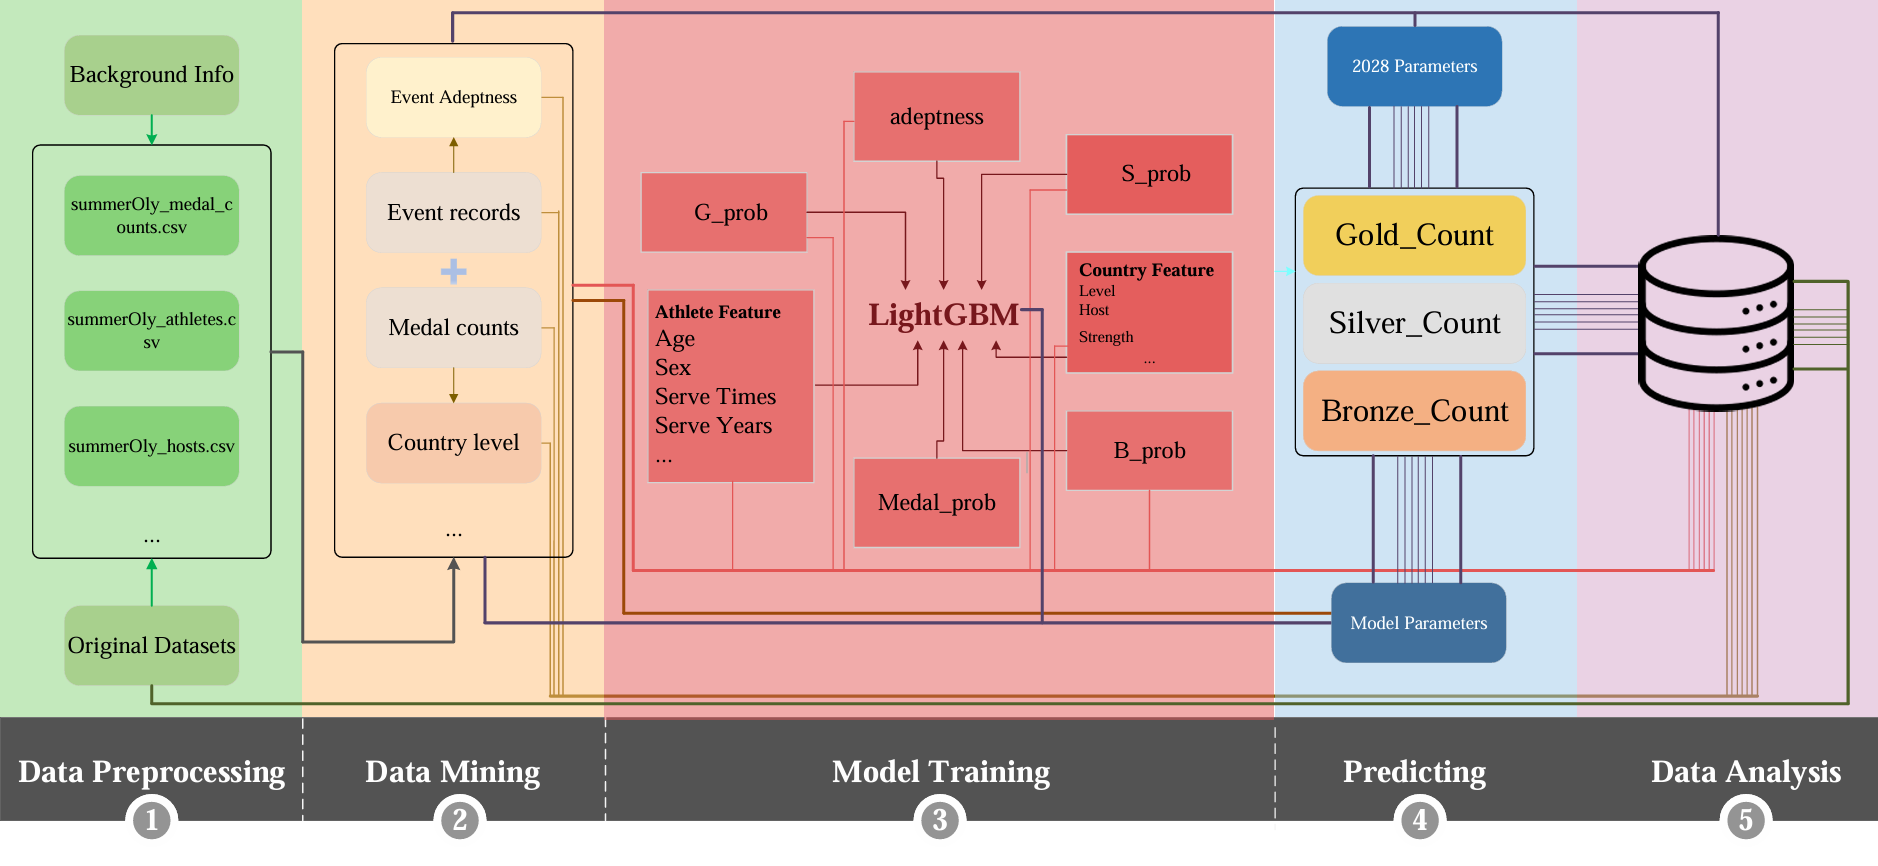
\includegraphics[width=16cm]{img/da.png}
	\caption{Workflow of Our Methodology}
	\label{fig:aa}
\end{figure}


\section{Question Preparation}
\subsection{Assumptions}
\textbf{Assumption 1 } \textit{The number of medals won by each country typically fluctuates only slightly from year to year, without significant increases or decreases.}

The total medal count of a country more accurately reflects the long-term investments and developmental outcomes in sports, rather than short-term results that can be drastically altered. Furthermore, \textbf{external factors} that influence medal counts, such as the organization of international competitions, rule changes, and judging standards, tend to remain relatively stable in the short term.


\textbf{Assumption 2 } \textit{Each year, a number of new athletes join the Olympic Games, some of whom may be competing for the first time. The specific proportion of these athletes wDue to the systematic nature of athlete training and the relative consistency of competition environments, their performance tends to remain stable. By mitigating the impact of outliers, the model can avoid being influenced by extreme values.  ill be estimated through our simulation. }

Due to the inclusion of new athletes each year and the replacement of older ones, in order to predict the medal count for the next Olympic Games, we need to simulate the new athletes based on historical athlete data using algorithms.


\textbf{Assumption 3} \textit{ The performance variability of athletes is assumed to be limited, with minimal occurrences of exceptional overperformance or underperformance.  }

The performance variability of athletes is assumed to be limited, with minimal occurrences of exceptional overperformance or underperformance.  


\subsection{Notations}

The primary notations used in this paper are listed in Table \ref{tb:notation}.

% 三线表示例

	
	\begin{longtable}{cl}
		\caption{Notations}\label{tb:notation} \\
		\toprule
		\multicolumn{1}{m{4cm}}{\centering Symbol}
		&\multicolumn{1}{m{13cm}}{\centering Definition}\\
		\midrule
		\endfirsthead
		
		\multicolumn{2}{c}%
		{\tablename\ \thetable\ -- \textit{Continued from previous page}} \\
		\toprule
		\multicolumn{1}{m{3cm}}{\centering Symbol}
		&\multicolumn{1}{m{8cm}}{\centering Definition}\\
		\midrule
		\endhead
		
		\midrule
		\multicolumn{2}{r}{\textit{Continued on next page}} \\
		\endfoot
		
		\bottomrule
		\endlastfoot
		
		$C_{i}$&Certain country\\
		$E_{i}$&Specific event\\
		$G$&Gold medal count\\
		$V$&Silver medal count\\
		$B$&Bronze medal count\\
		$M$&Total count of the 3 types of medals\\
		$A$&Number of new medals\\
		$T$&Times of Olympic participations\\
		$T$&Total count of events\\
		$\gamma$&Sport Advantage Coefficient\\
		$ m_{C_{i}}$ &Total medal count of a certain country\\
		$ m_{C_{i},E_{j}}$ &Total medal count of a certain country in a specific event\\
		$L_{i}$&Country clustering level\\
		$g_{i}$&the second one\\
		$X$&Historical total medal counts (gold, silver, and bronze) of all countries\\
		$\xi$&The Probability of First Medal\\
		$\sigma$&Standard deviation\\
		$\kappa$&Normalized version of probability of first medal\\
	\end{longtable}
	
\section{Data Preprocessing}
\subsection{Basic Data Preprocessing}
Due to the diverse factors influencing competition outcomes, there are significant differences in the competitive levels of countries in the Olympic Games, which have been reflected in past competitions, specifically in the total number of gold, silver, and bronze medals won by each country. 

To demonstrate the differences in the levels of countries in previous Olympic Games (i.e. national level), we employed the \textbf{KMeans++} algorithm. Based on the number of gold, silver, and bronze medals, as well as the total medal count of each country in past Olympics, we categorized the countries into five levels. These 5 levels, L1, L2, L3, L4, and L5, form a partition of the sample set X (the total number of gold, silver, and bronze medals won by countries in previous Olympic Games).
\begin{equation}
G_{i} \cap G_{j}=\emptyset, \bigcup_{i=1}^{5} G_{i}=X
\end{equation}
After the classification, the distribution of countries across the 5 levels is shown in the figures:
\begin{figure}[H]
	\centering
	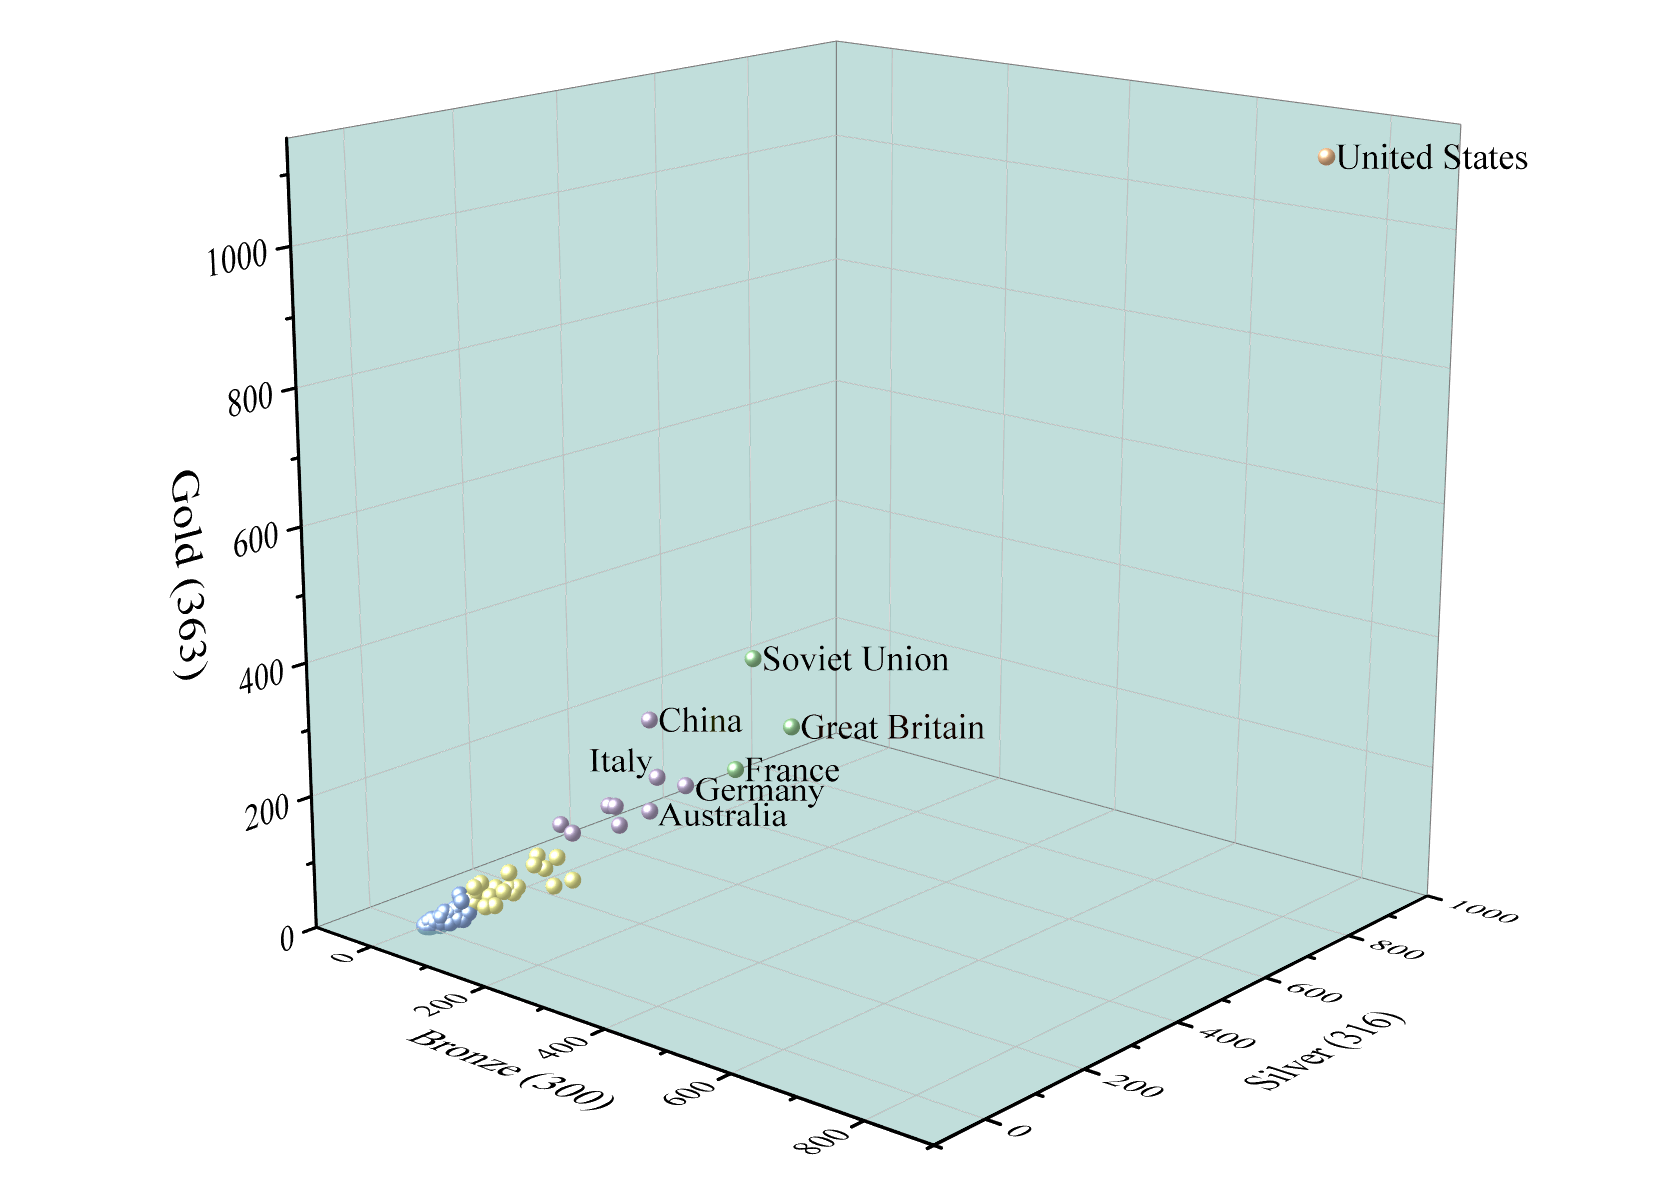
\includegraphics[width=12cm]{img/Level1.png}
	\caption{Scatter plot of national level classification (based on KMeans++ clustering algorithm)}
	\label{fig:aa}
\end{figure}

\begin{figure}[H]
	\centering
	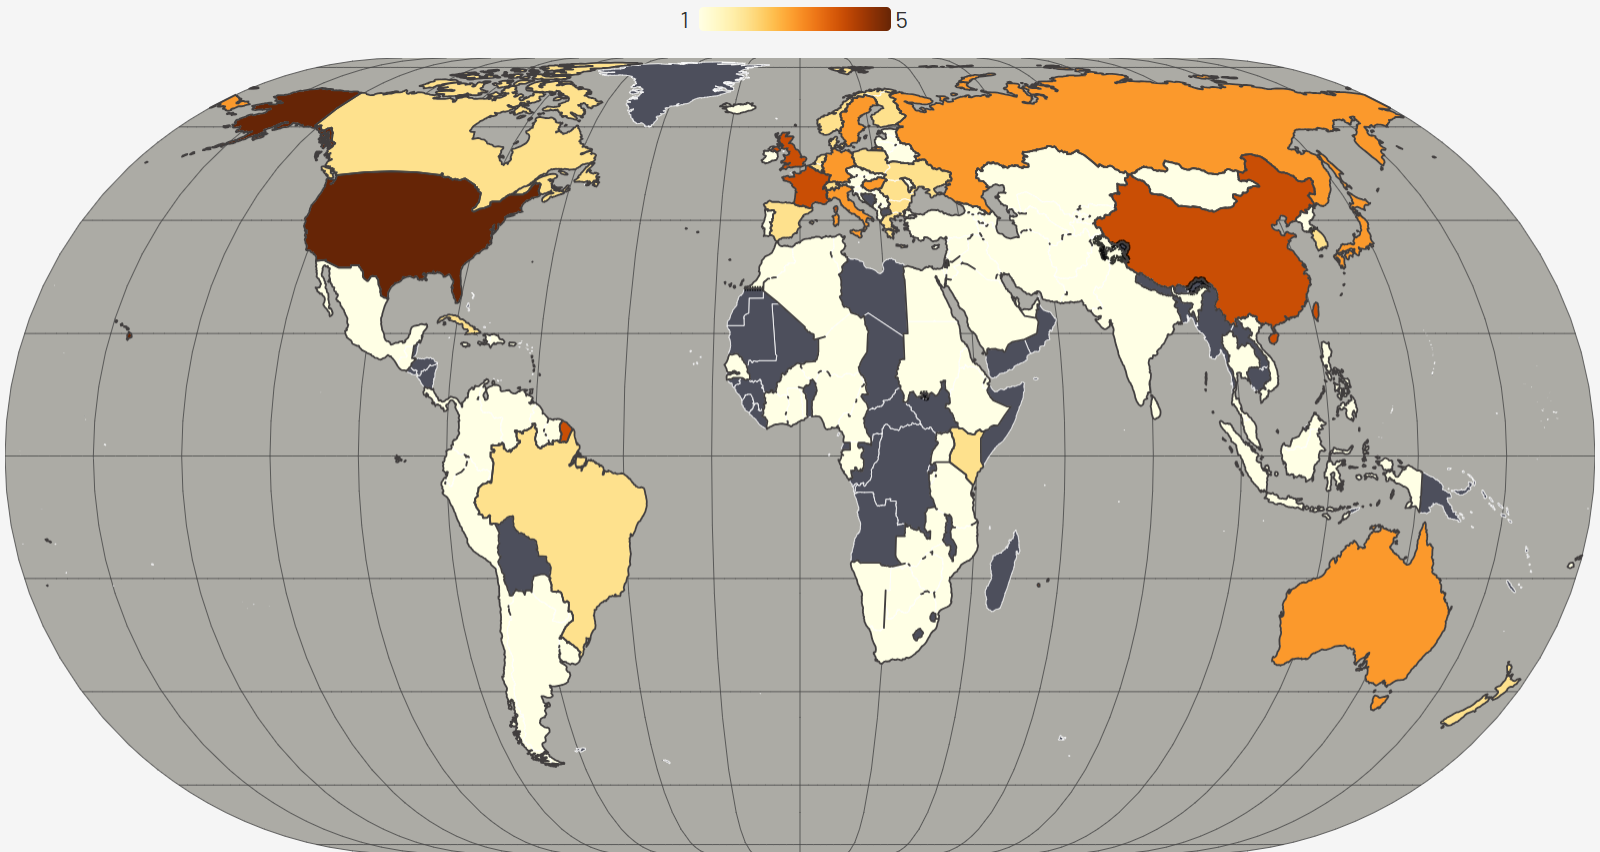
\includegraphics[width=12cm]{img/Level2.png}
	\caption{Geographical Distribution Map of Country Level Classification}
	\label{fig:aa}
\end{figure}


In addition, we created 10 new features based on the original variables, which were utilized during the modeling process with the \textbf{LightGBM} model.

%Table 2 :变量名表 Variable Name
\begin{longtblr}[
	caption = {Variable Name},
	]{
		vline{1-4} = {1-10}{},
		hline{1-11} = {1-3}{},
	}
	Variable Name                                                    & \textit{Code}                                                & Definition                                                                      &  \\
	Whether~Host Country                                             & \textit{is host}                                             & {Whether the country is the host(1 for host,0 for\\~non-host)}                  &  \\
	{Medal Expectation\\Increment *Personnel\\Expectation lncrement} & {\textit{medal\_increment *}\\\textit{personnel\_increment}} & {Product of medal\\expectation increment and\\personnel expectation\\increment} &  \\
	{Sport Advantage\\Coefficient}                                 & \textit{sport\_adv}                                           & {Advantage coefficient of\\a specific sport}                                  &  \\
	Country Level                                                    & \textit{country\_lvl}                                        & {The level of the country in the competition\\(ordered by rank)}                &  \\
	{Project Medal\\Expectation /Project\\Personnel Expection~}                         & \textit{sport\_medal \_per\_ person}                          & {Ratio of sport medals to projected personnel\\for a specific sport}          &  \\
	Gold Medal Probability                                           & \textit{gold\_prob}                                          & {Probability of an athlete~\\winning a gold medal}                              &  \\
	{Silver Medal\\Probability}                                      & \textit{silver\_prob}                                        & Probability of an athlete~ winning a silver medal                               &  \\
	{Bronze Medal\\Probability}                                      & \textit{silver\_prob}                                        & Probability of an athletewinning a bronze medal                                 &  \\
	No Medal Probability                                             & \textit{no\_medal\_probe}                                    & Probability of an athlete winning no medal                                      &  \\
	&                                                              &                                                                                 &  \\
	&                                                              &                                                                                 &  
\end{longtblr}




\subsection{Data Mining}
\subsubsection{Participant List Prediction}
To predict future scenarios, we analyzed the trends in the number of participants for each country, event and year, and applied \textbf{Linear Regression} for fitting.

\begin{figure}[H]
	\centering
	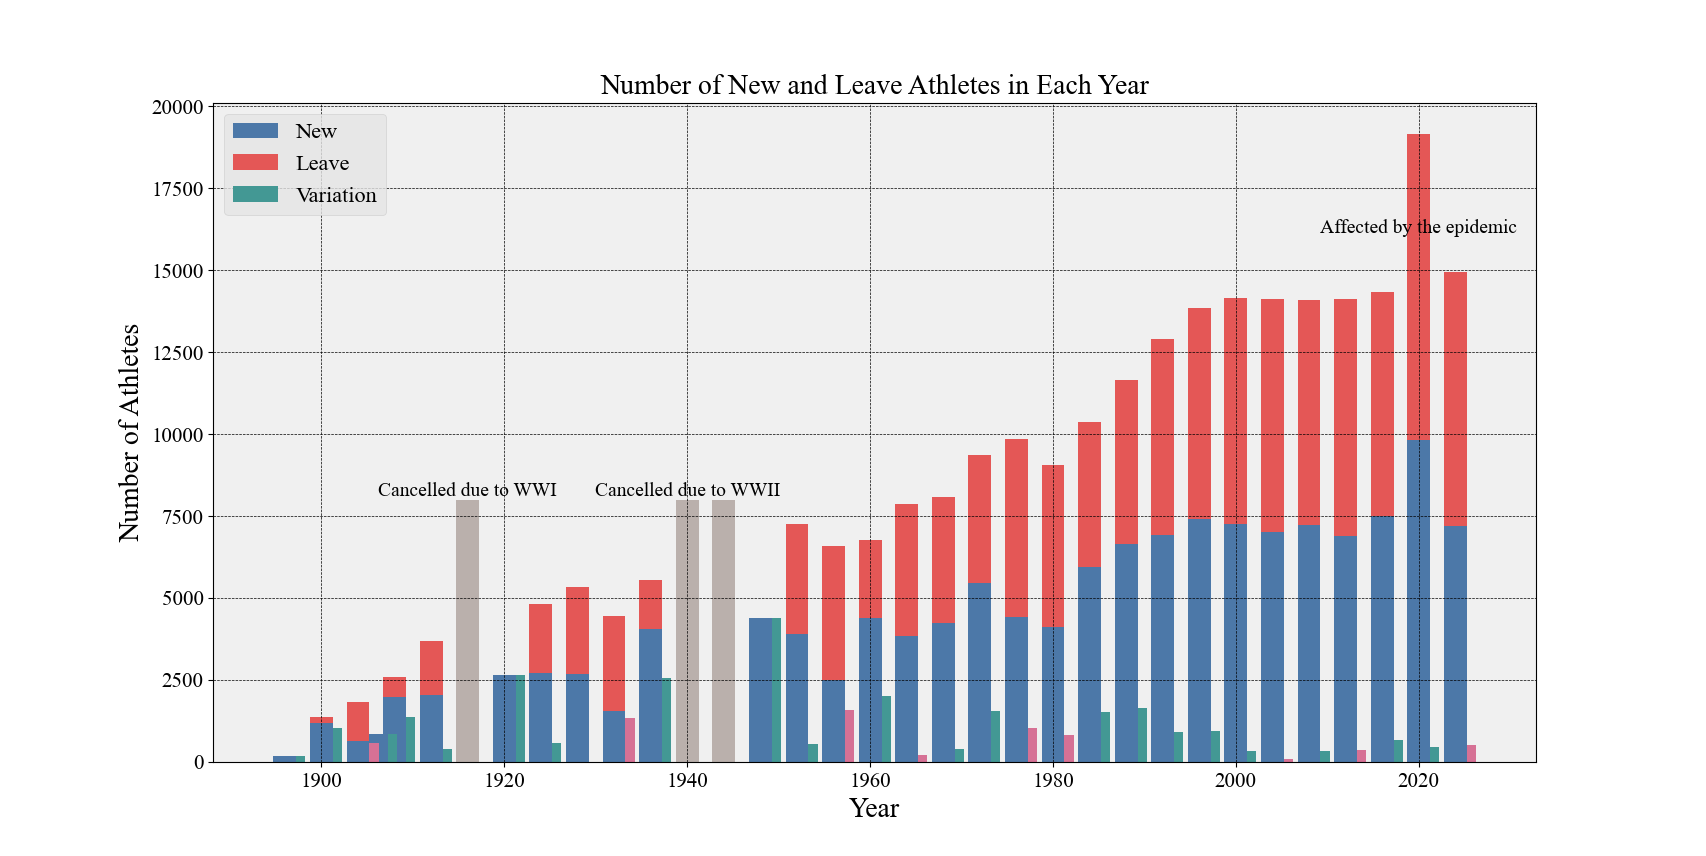
\includegraphics[width=12cm]{img/Number.png}
	\caption{Number of New and Leave Athletes in Each Year}
	\label{fig:aa}
\end{figure}

Then, we compiled the distribution of the times of participations and the distribution of athlete tenure based on historical data, as shown in the figure.
\begin{figure}[H]
	\centering
	\begin{subfigure}[b]{.48\textwidth}
		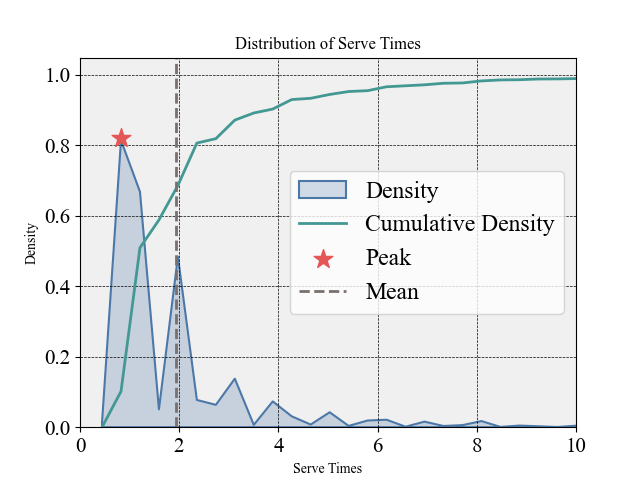
\includegraphics[width=\textwidth]{img/Times.png}
		\caption{Distribution of Serve Times}\label{subfig:left}
	\end{subfigure}
	\begin{subfigure}[b]{.51\textwidth}
		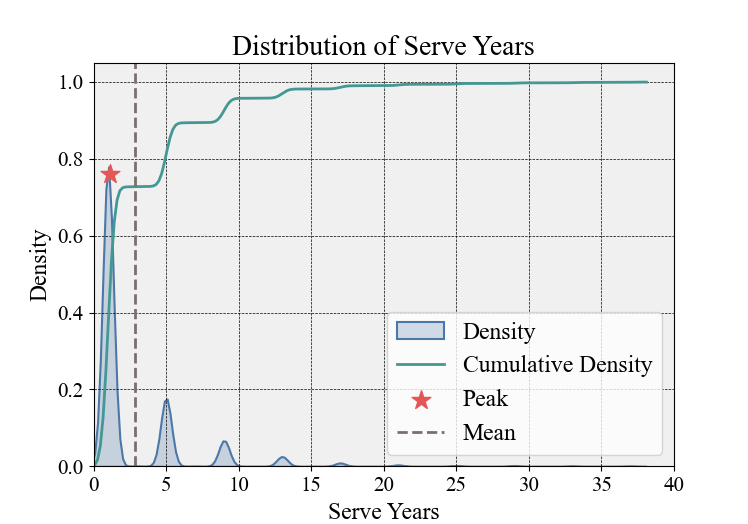
\includegraphics[width=\textwidth]{img/Years.png}
		\caption{Distribution of Serve Years}\label{subfig:right}
	\end{subfigure}
	\caption{Athlete Service Status}\label{fig:subfigures}
\end{figure}


From the distribution chart, it can be seen that nearly \( 80\% \) of athletes have participated in 1 or 2 matches, with the average number of serve times being 1.94, meaning each athlete participates in approximately 2 matches. Based on this assumption, we consider that each participating athlete will compete in \textbf{2 matches on average}. Additionally, around \( 80\% \) of athletes have participated in only 1 Olympic Games, while nearly \( 20\% \) have participated in 2. Therefore, we can assume that \( 20\% \) of the veteran athletes will continue to compete in the next Olympic Games, providing a basis for determining which athletes will continue to participate.

To predict the Participant List, we employed Monte Carlo simulation, which consisted of two parts: the first part involved selecting \( 20\% \) of veteran athletes to continue competing (\( 20\% \) conforming to the original data distribution), while the second part generated new random athletes based on historical athlete data.

In the previous sections, we determined which athletes will continue to compete. To simulate new random athletes, we simplified each individual into three parameters: the probabilities of winning a gold, silver, or bronze medal.

For a given country in a specific event, the average number of medals won by all athletes serves as the standard number of medals for a representative athlete. The medal expectations were categorized into 3 scenarios: \textbf{optimistic}, \textbf{moderate}, and \textbf{pessimistic}. The optimistic expectation was calculated by averaging the top \( 50\% \) of the team, the moderate expectation by averaging all team members, and the pessimistic expectation by averaging the bottom \( 50\% \).

Using the Previous Participants' Records as the basis for Monte Carlo simulation, we ultimately determined the Participant List Prediction.



\subsubsection{Distribution of Countries' Adept Sports}
Due to factors such as cultural and geographical environments, countries exhibit distinct advantages in different events. For example, Kenya and Ethiopia excel in long-distance running, particularly in Athletics, largely due to the training conditions in high-altitude regions. Brazil, with its deep football culture, has produced many world-class players, a result of its warm climate and environment conducive to year-round outdoor sports.

By analyzing the performance of various countries in different events across past Olympic Games, we extracted a feature variable $\gamma$ (\textbf{Event Adeptness Coefficient}), to represent the advantages of these countries in certain events.

%公式
\begin{equation}
	\gamma = \frac{m_{C_i,E_j}}{\sum m_{C_i,E_j}}
\end{equation}





By extracting features, we mined the level of expertise of each country in different events within the dataset, such as China's performance across various events, as shown in the figure below:

\begin{figure}[H]
	\centering
	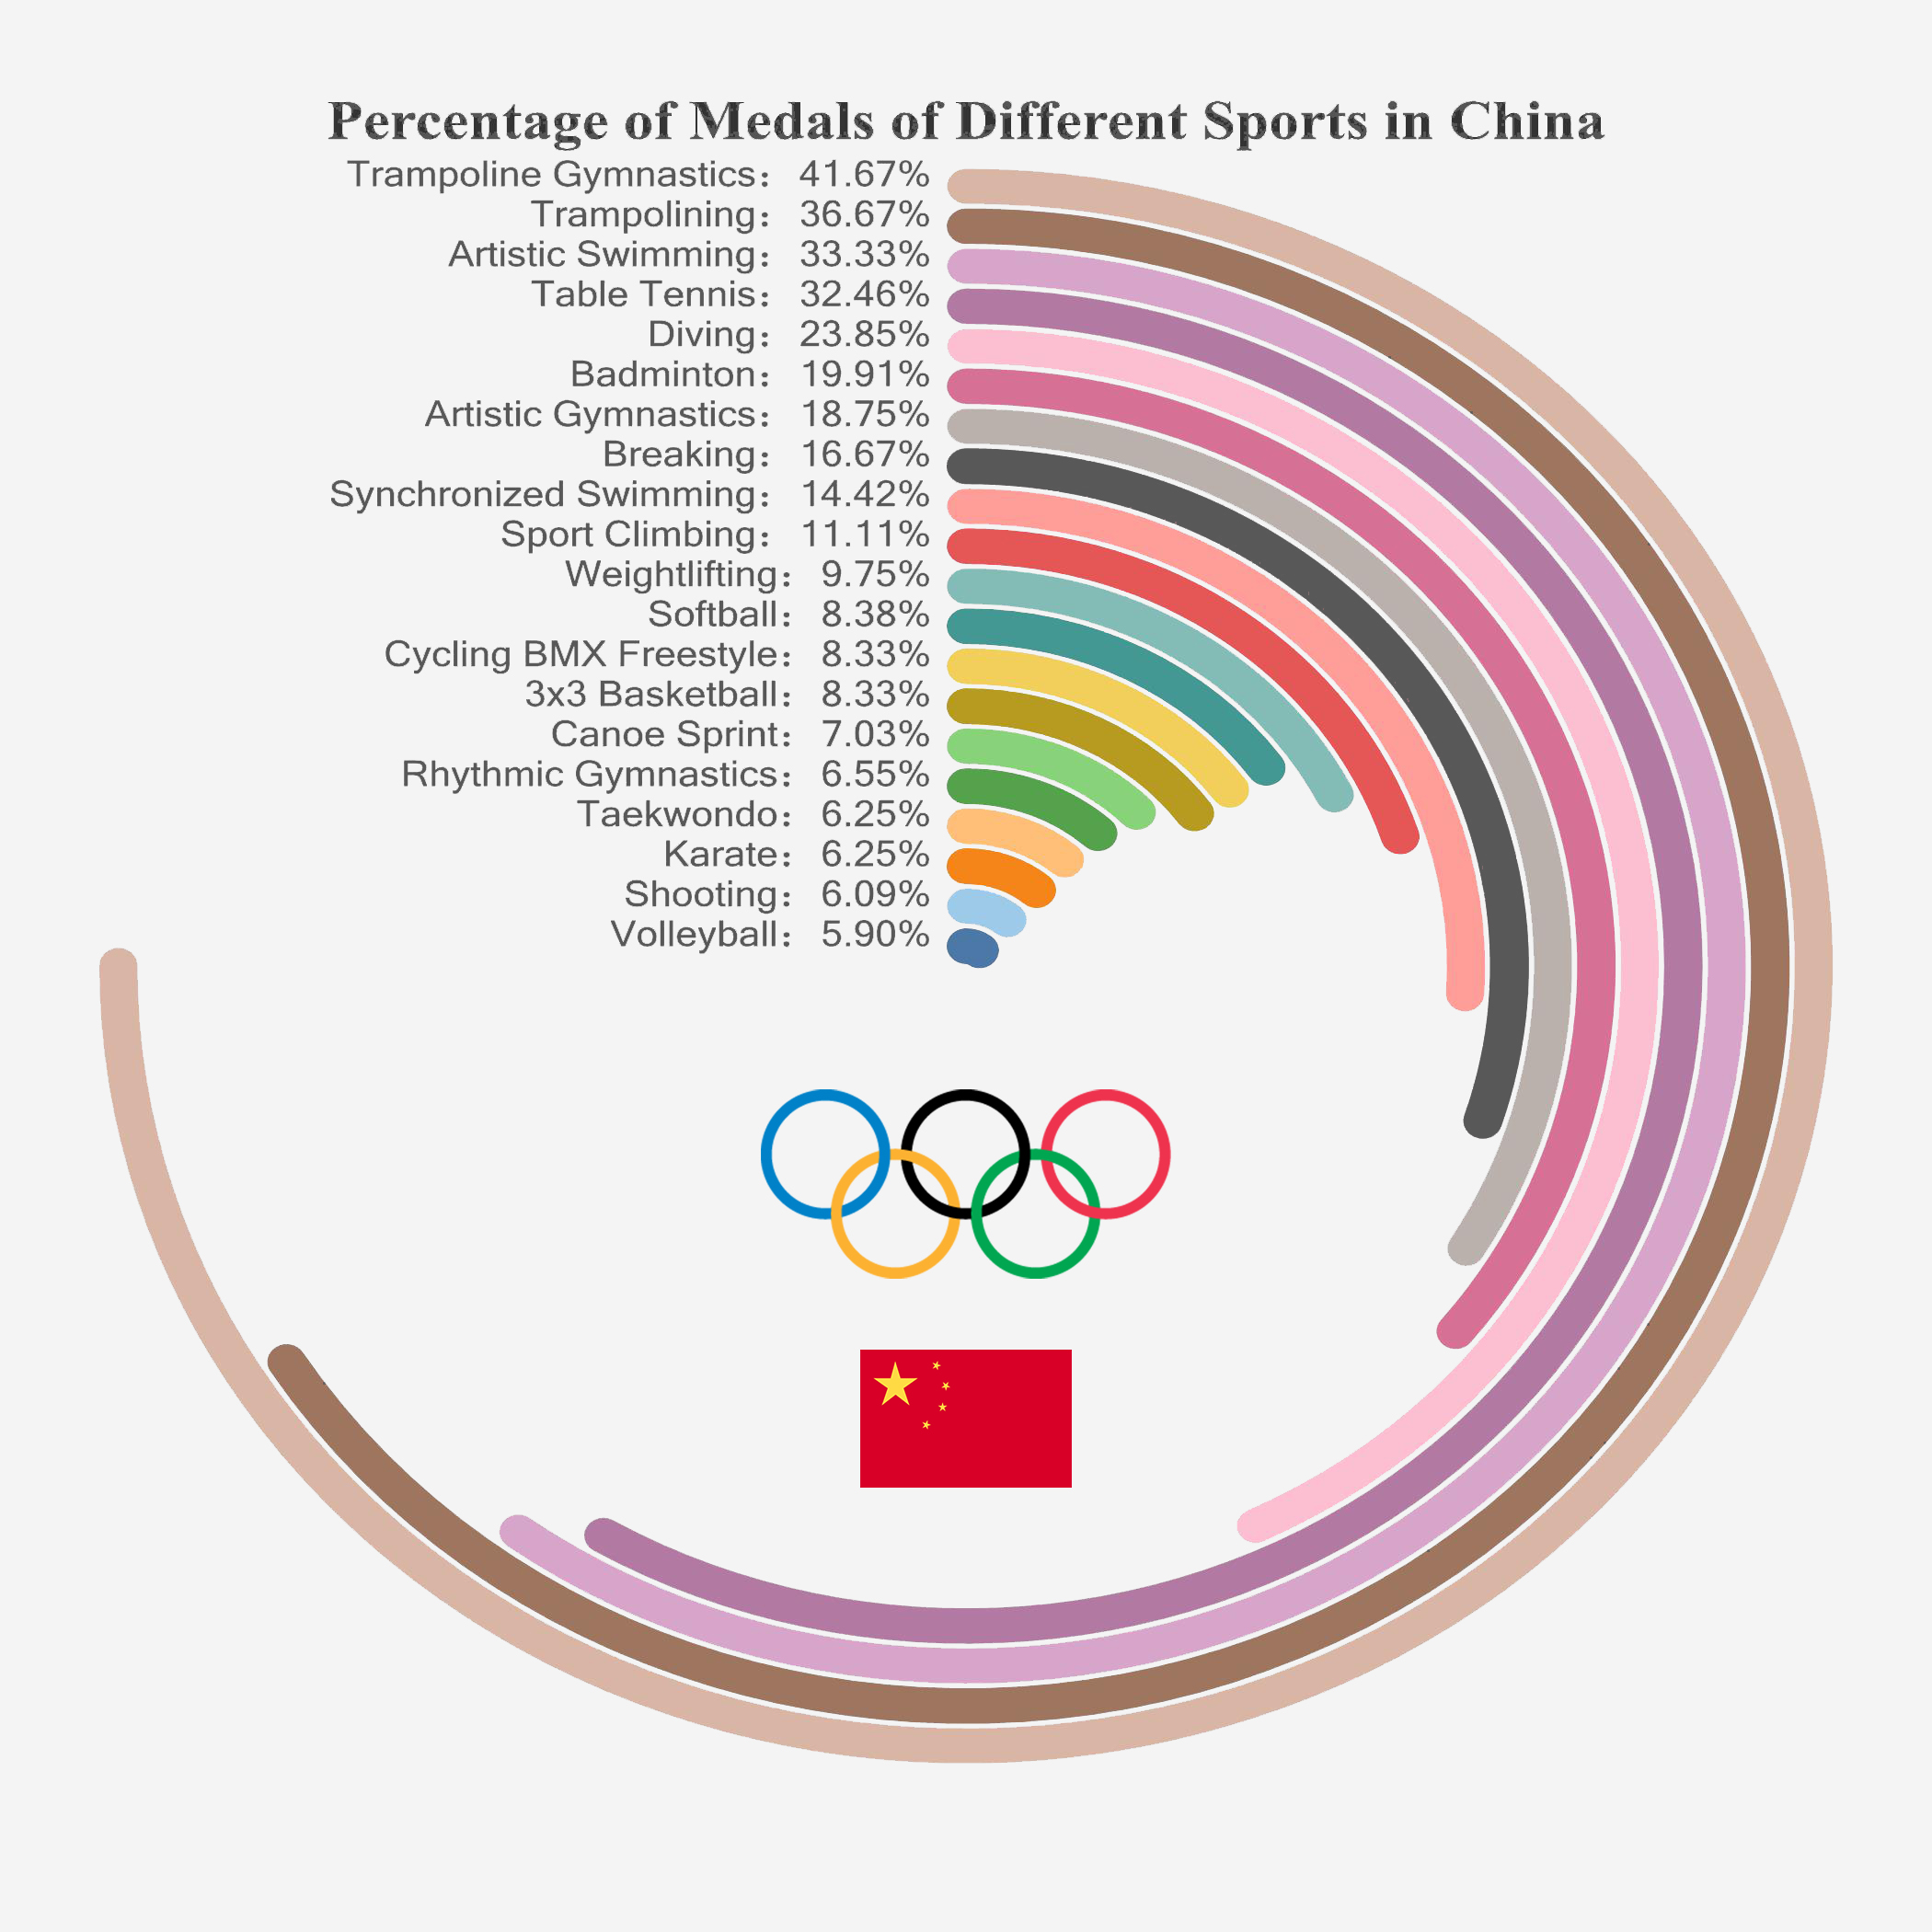
\includegraphics[width=8cm]{img/Percentage.jpg}
	\caption{Percentage of Medals of Different Sports in China}
	\label{fig:aa}
\end{figure}


\subsubsection{Changes in Medal Count}
Since the IOC makes adjustments to events each year, the total number of medals awarded in each event does not remain exactly the same each year. To address this, we applied\textbf{ Linear Regression} to fit the number of gold, silver, and bronze medals awarded in each event across past Olympic Games and predicted the medal distribution for the upcoming Olympic Games, providing a reference for subsequent operations.

\section{Task1:Medal Prediction Model Based on LightGBM}
\subsection{Medal Table}
The medal table is influenced by various factors. To predict the standings for the next Olympics, we considered key factors identified during data preprocessing, such as nation level, participating athletes, country-specific event strengths, and adjustments to medal counts.

Additionally, we accounted for the host country's advantage, including whether a country is the host or hosting for the first time, categorizing and quantifying this factor into three categories for the model. These five factors were collectively termed \textbf{National Background Factors}.

% \usepackage{longtable}


\begin{longtable}{|c|c|} 
	\hline
	Category & Definition               \endfirsthead 
	\hline
	0        & Not host                 \\ 
	\hline
	1        & Host for the 1st time    \\ 
	\hline
	2        & Host for more than once  \\
	\hline
\end{longtable}


And the steps of our \textbf{LightGBM} model are as below:
\begin{figure}[H]
	\centering
	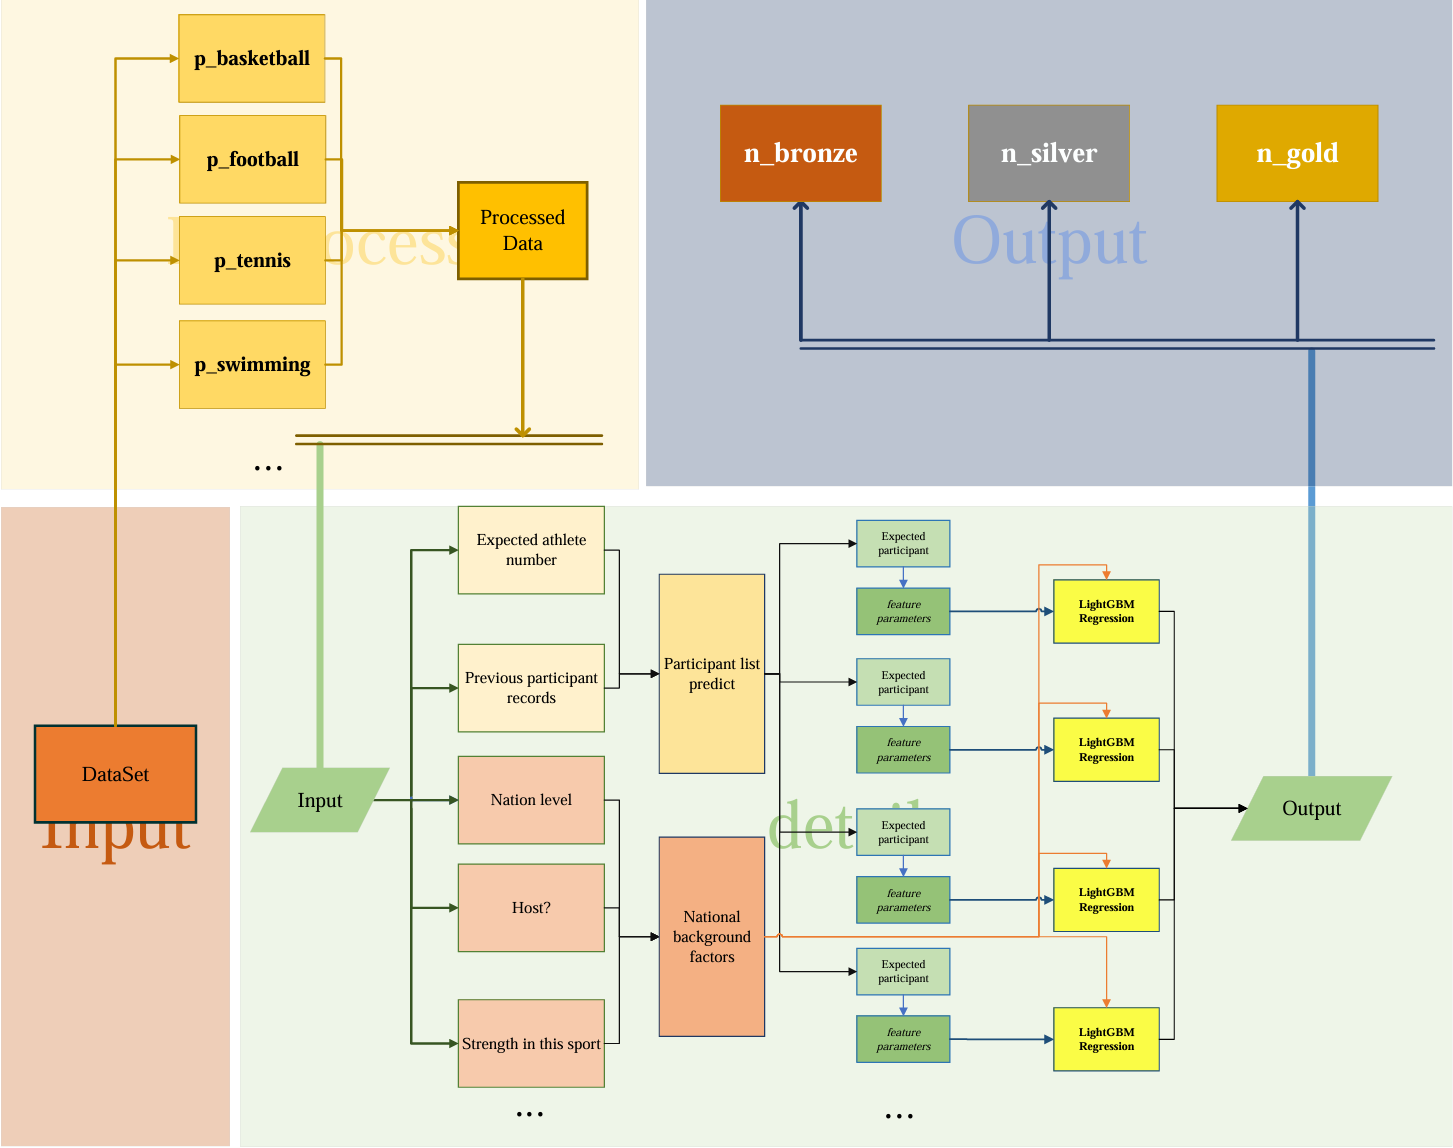
\includegraphics[width=11cm]{img/xiao.png}
	\caption{LightGBM Model Flow Chart}
	\label{fig:aa}
\end{figure}
The prediction of the Olympic medal table is essentially a multi-task learning problem, with the goal of predicting the number of gold, silver, and bronze medals each country is likely to win in different events. To accomplish this task, we need to input a large and diverse set of data while outputting predictions for multiple medal categories. These features are highly suitable for the LightGBM model.

Building on \textbf{GBDT}, LightGBM accelerates the computation using histograms, optimizing training efficiency and enabling the fast processing of high-dimensional, sparse, large-scale data. Compared to traditional logistic regression, LightGBM can capture \textbf{nonlinear relationships} through tree splitting, offering a performance advantage in accurately handling complex data and nonlinear relationships, significantly improving accuracy. Additionally, it can automatically handle missing values, providing great convenience for data preprocessing.

As a gradient boosting-based regression model, in LightGBM, the objective function consists of two parts: the loss function and the regularization term.

\begin{equation}
	\mathcal{L} = \sum_{i=1}^{n} L(y_i, \hat{y}_i^{(m-1)} + \eta f_m(x_i)) + \Omega(f_m)
\end{equation}

The optimized loss function based on GBDT is represented as \textbf{squared error} in the medal prediction regression task.

$y_i$ denotes the true value.
$\hat{y}_i^{(m-1)}$ is the current model's predicted value.
$\hat{y}_i^{(m-1)}$ +$\eta f_m(x_i)$ is the model's predicted value at the m-th step during the gradient boosting model update process.
$\Omega(f_m)$ is the regularization term, which prevents overfitting of the model and controls the complexity of the trees.

We input the previously obtained data into LightGBM for iterative model training. After training, we input the factors affecting the predictions for the next edition into the model, ultimately obtaining the predicted medal table for the 2028 Summer Olympics in Los Angeles, USA, are shown in Figure \ref{fig:aa}.
%奖牌榜预测图
\begin{figure}[H]
	\centering
	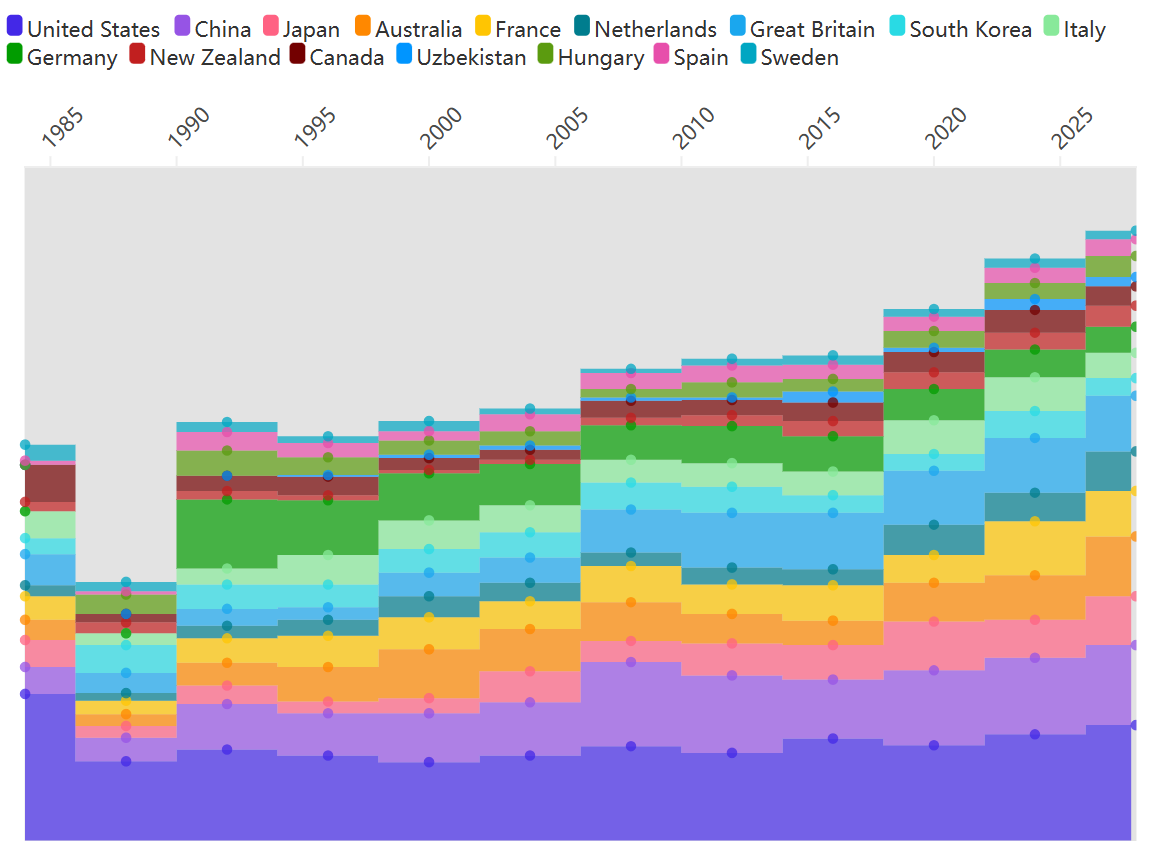
\includegraphics[width=11cm]{img/Predict.png}
	\caption{Medal Count Prediction}
	\label{fig:aa}
\end{figure}


According to the model's predictions, the United States is expected to see a significant increase in medal count compared to the previous year, while France will experience a notable decrease, which is related to the \textbf{home-field advantage} of the host country. Additionally, due to changes in the number of medals for certain events, the medal counts for Australia, Japan, and the Netherlands are expected to rise, while Italy and South Korea will see a decline. China's medal count is projected to remain relatively stable.

To more accurately simulate the actual number of medals won, we simplify each individual into 3 parameters: \textbf{the probabilities of winning gold, silver, and bronze medals}. For a specific country and event, the average number of medals won by all team members represents the probability that a standard "virtual athlete" should have.

For the expected outcomes, the optimistic expectation is calculated by averaging the top \( 50\% \) of the team, the moderate expectation is based on the average of all team members, and the pessimistic expectation is derived by averaging the bottom \( 50\% \) of the team.

The "Previous Participants Record" serves as the basis for the Monte Carlo simulation, which consists of two parts: the first part involves selecting \( 20\% \) of veteran athletes to continue competing (with \( 20\% \) corresponding to the original data distribution), and the second part uses historical athlete data to generate new random athletes.


\begin{figure}[H]
	\centering
	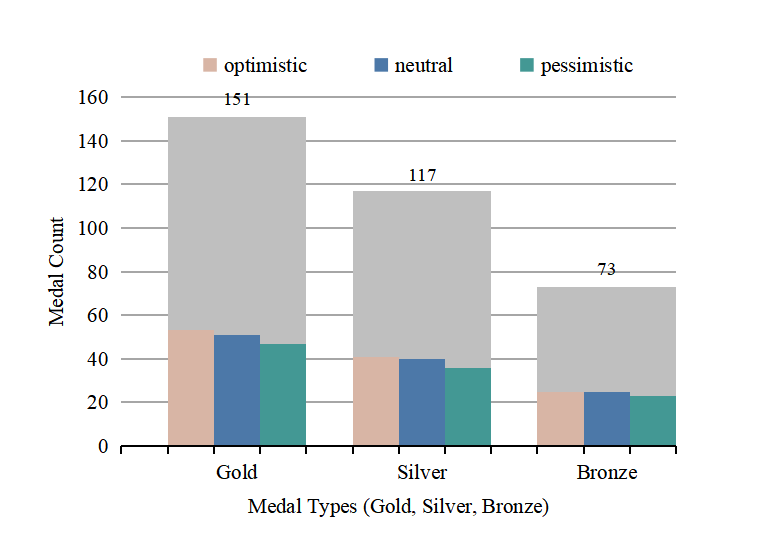
\includegraphics[width=12cm]{img/OP1.png}
	\caption{USA Medal Count Prediction}
	\label{fig:USA}
\end{figure}


Based on the model, we predict the medal outcomes for each country in the 2028 Olympic Games. A partial result is provided here, with the full version available in the appendix. The predicted outcomes for the United States are presented, showing that, overall, the optimistic expectation > moderate expectation > pessimistic expectation. 
\begin{longtable}{l|c|c|c|c|c|c|c|c|c|c}
\caption{Countries' Medal Count Prediction(part)}\\
	Country              & \multicolumn{1}{l|}{\begin{tabular}[c]{@{}l@{}}G\_\\pes.\end{tabular}} & \multicolumn{1}{l|}{\begin{tabular}[c]{@{}l@{}}S\_\\pes.\end{tabular}} & \multicolumn{1}{l|}{\begin{tabular}[c]{@{}l@{}}B\_\\pes.\end{tabular}} & \multicolumn{1}{l|}{\begin{tabular}[c]{@{}l@{}}G\_\\opt.\end{tabular}} & \multicolumn{1}{l|}{\begin{tabular}[c]{@{}l@{}}S\_\\opt.\end{tabular}} & \multicolumn{1}{l|}{\begin{tabular}[c]{@{}l@{}}B\_\\opt.\end{tabular}} & \multicolumn{1}{l|}{Gold} & \multicolumn{1}{l|}{Silver} & \multicolumn{1}{l|}{Bronze} & \multicolumn{1}{l}{Total}  \endfirsthead 
	\hline
	United States        & 47                                                                     & 36                                                                     & 23                                                                     & 53                                                                     & 41                                                                     & 25                                                                     & 51                        & 40                          & 25                          & 117                        \\ 
	\hline
	China                & 35                                                                     & 35                                                                     & 15                                                                     & 46                                                                     & 38                                                                     & 20                                                                     & 40                        & 36                          & 17                          & 95                         \\ 
	\hline
	Australia            & 28                                                                     & 20                                                                     & 22                                                                     & 33                                                                     & 24                                                                     & 24                                                                     & 29                        & 22                          & 23                          & 71                         \\ 
	\hline
	France               & 23                                                                     & 19                                                                     & 19                                                                     & 27                                                                     & 20                                                                     & 22                                                                     & 24                        & 19                          & 21                          & 64                         \\ 
	\hline
	Germany              & 18                                                                     & 24                                                                     & 14                                                                     & 23                                                                     & 26                                                                     & 16                                                                     & 21                        & 25                          & 15                          & 61                         \\ 
	\hline
	United Kingdom       & 20                                                                     & 19                                                                     & 14                                                                     & 26                                                                     & 24                                                                     & 15                                                                     & 25                        & 21                          & 15                          & 61                         \\ 
	\hline
	Japan                & 16                                                                     & 25                                                                     & 14                                                                     & 19                                                                     & 27                                                                     & 16                                                                     & 17                        & 26                          & 16                          & 58                         \\ 
	\hline
	Italy                & 15                                                                     & 20                                                                     & 15                                                                     & 17                                                                     & 20                                                                     & 22                                                                     & 16                        & 20                          & 16                          & 53                         \\ 
	\hline
	Spain                & 21                                                                     & 10                                                                     & 13                                                                     & 30                                                                     & 12                                                                     & 14                                                                     & 25                        & 12                          & 13                          & 50                         \\ 
	\hline
	Netherlands          & 24                                                                     & 6                                                                      & 13                                                                     & 29                                                                     & 9                                                                      & 15                                                                     & 26                        & 8                           & 15                          & 47                         \\ 
	\hline
	New Zealand          & 20                                                                     & 13                                                                     & 9                                                                      & 22                                                                     & 15                                                                     & 10                                                                     & 22                        & 14                          & 9                           & 45                         \\ 
	\hline
	...                  & ..                                                                     & ..                                                                     & ..                                                                     & ..                                                                     & ..                                                                     & ..                                                                     & ..                        & ..                          & ..                          & ..                         \\
	\multicolumn{1}{l}{} & \multicolumn{1}{c}{}                                                   & \multicolumn{1}{c}{}                                                   & \multicolumn{1}{c}{}                                                   & \multicolumn{1}{c}{}                                                   & \multicolumn{1}{c}{}                                                   & \multicolumn{1}{c}{}                                                   & \multicolumn{1}{c}{}      & \multicolumn{1}{c}{}        & \multicolumn{1}{c}{}        &                           
\end{longtable}
%4.2
\subsection{Countries that Win Their First Medal}
Since the model used for predicting the medal table in the previous section yields varying levels of accuracy for countries of different rankings, the predictions for higher-ranked countries, such as the United States and China, are more accurate. In contrast, the prediction errors for lower-ranked countries are larger. Clearly, countries that have not yet won medals fall into the category with higher prediction errors, so the previous model is not applicable in this case.

Therefore, for countries that have never won a medal before, we calculate their \textbf{first medal index} $\xi$.

\begin{equation}
	\xi = \sum_{i=1}^{n} \left( T_{E_i} \ast A_{E_i} \right)
\end{equation}





The number of competitions is counted from the original dataset, and the expected increase in the number of medals for the next edition is predicted through a \textbf{Linear Regression model} based on historical data.

As the number of competitions and the expected increase in medals for the next edition increase for countries that have not won medals, the likelihood of these countries winning medals becomes higher. Therefore, the first medal index $\xi$ is positively correlated with the probability of a country that has not won a medal securing its first medal in the next Olympic Games, meaning that the larger the $\xi$ value, the higher the likelihood of winning the first medal.

In order to visualize the accuracy of a country's first medal prediction, we normalized the first medal index using the \textbf{Z-score} and then multiplied it by 0.8 to obtain the first medal coefficient $\kappa$.

\begin{equation}
	\kappa = 0.8 \times \frac{\xi - \overline{\xi}}{\sigma}
\end{equation}

Here,$\overline{\xi}$ refers to the mean of the original data, and $\sigma$ refers to the standard deviation of the original data.
The calculated results are shown in Figure \ref{fig:First Medal}:
%首奖可能性图
\begin{figure}[H]
	\centering
	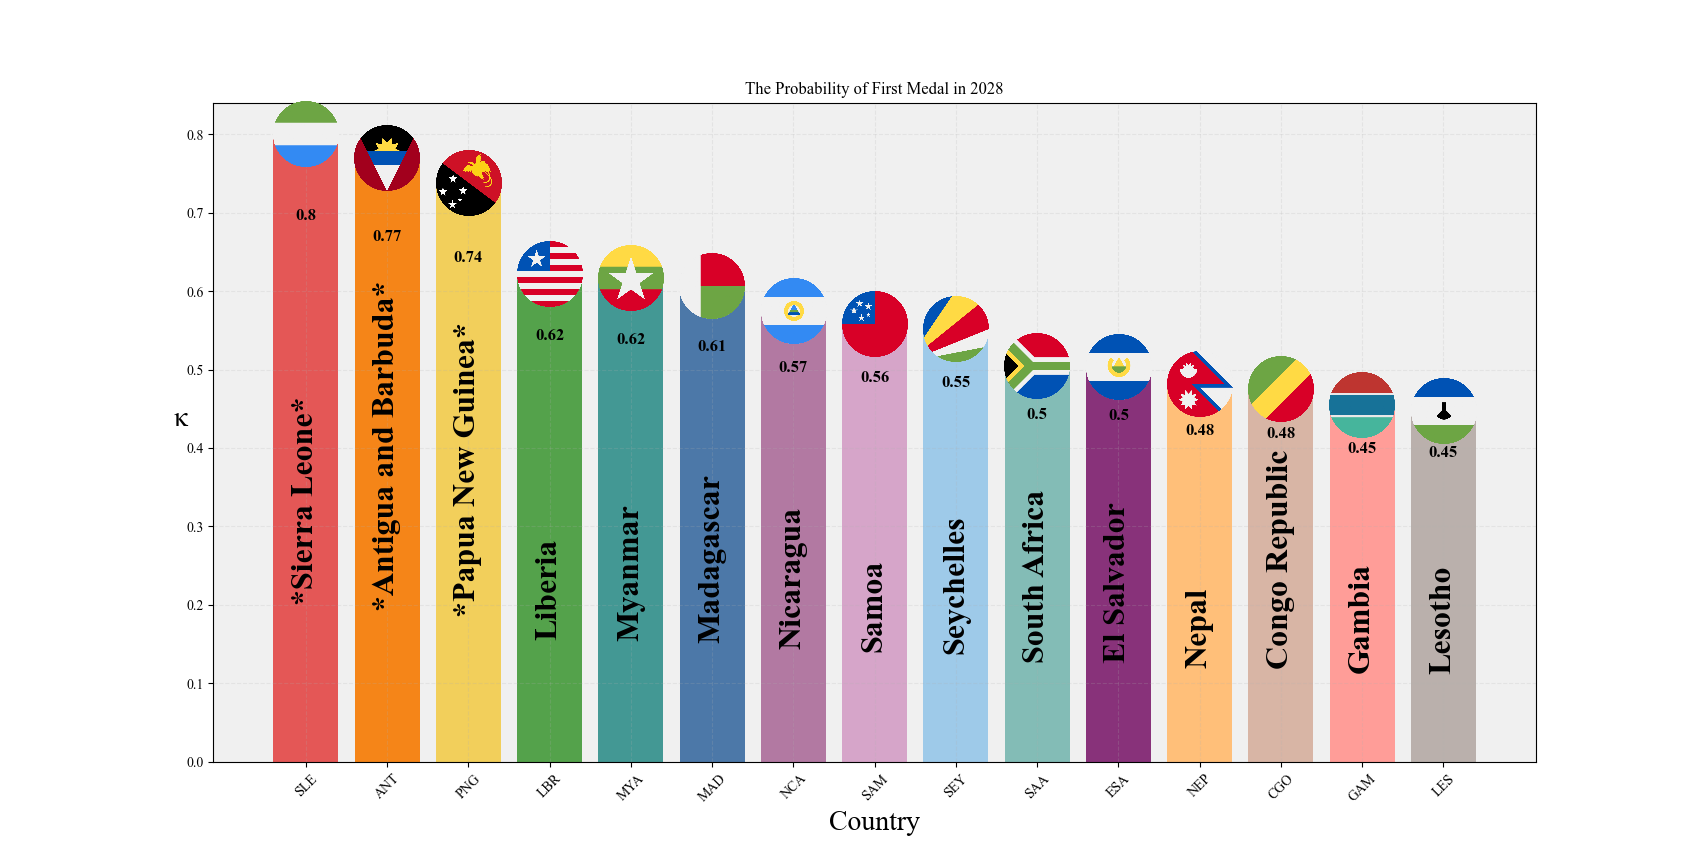
\includegraphics[width=16cm]{img/First.png}
	\caption{The Probability of First Medal in 2028}
	\label{fig:First Medal}
\end{figure}


As shown in the figure, \textbf{Sierra Leone (SLE)}, \textbf{Antigua and Barbuda (ANT)}, and \textbf{Papua New Guinea (PNG)} are the three countries most likely to win their first medal in the next Olympic Games, with accuracies approximately 0.8, 0.77, and 0.74, respectively.


%4.3
\subsection{Events and Medal Counts by Countries}
In the data preprocessing section, we have calculated the adeptness of each country in each event, thus allowing us to roughly estimate the events in which each country excels.

We input the data of the dominant events of multiple countries into the prediction model and use \textbf{Spearman's Rank Correlation Coefficient} to analyze the correlation between the total medal count of a country and the medal count of a specific event, as well as the number of events in that event. This is because we cannot confirm that the data sample follows a normal distribution, nor can we ascertain that the relationship between the dominant events and the total medal count is linearly correlated. Spearman's Rank Correlation Coefficient is suitable for evaluating \textbf{nonlinear} relationships.

We studied the relationship between China's total medal count, gold medal count, and the number of awards and events in table tennis. For each pair of variables, we ranked the data points and assigned ranks to each data point. The rank difference for each data point is calculated as:

\begin{equation}
	d_i = R(X_i) - R(Y_i)
\end{equation}


Here, $d_i$ is the rank difference of the two variables for the i-th data point. 
Next, we compute the \textbf{Spearman's Rank Correlation Coefficient} ($R_s$). 

\begin{equation}
	R_s = 1 - \frac{6 \sum d_i^2}{n(n^2 - 1)}
\end{equation}


The absolute value of $R_s$ closer to 1 indicates a stronger correlation, while closer to 0 indicates a weaker correlation.A positive $R_s$ indicates a positive correlation between the two variables, meaning an increase in one variable typically accompanies an increase in the other. 

Through extensive data analysis, we identified 3 typical examples: table tennis in China, Athletics in Jamaica, and rowing in New Zealand, as shown in the figure.
%三个国家擅长项目的图
\begin{figure}[H]
	\centering
	\begin{subfigure}[b]{.3\textwidth}
		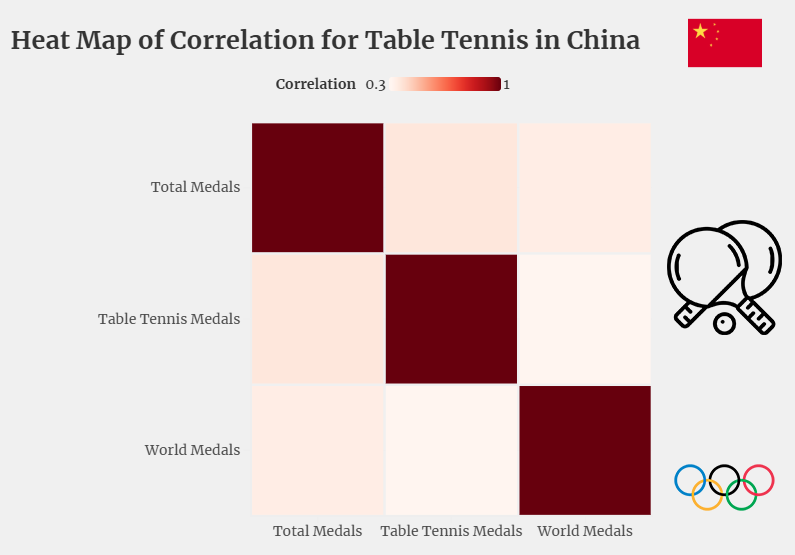
\includegraphics[width=\textwidth]{img/Table Tennis.png}
		\caption{Heatmap of Correlation for Table Tennis in China}\label{subfig:1}
	\end{subfigure}
	\hfill 
	\begin{subfigure}[b]{.33\textwidth}
		
\includegraphics[width=\textwidth]{img/Jamaica.png}
		\caption{ Heatmap of Correlation for Athletics in Jamaica}\label{subfig:2}
	\end{subfigure}
	\hfill 
	\begin{subfigure}[b]{.32\textwidth}
		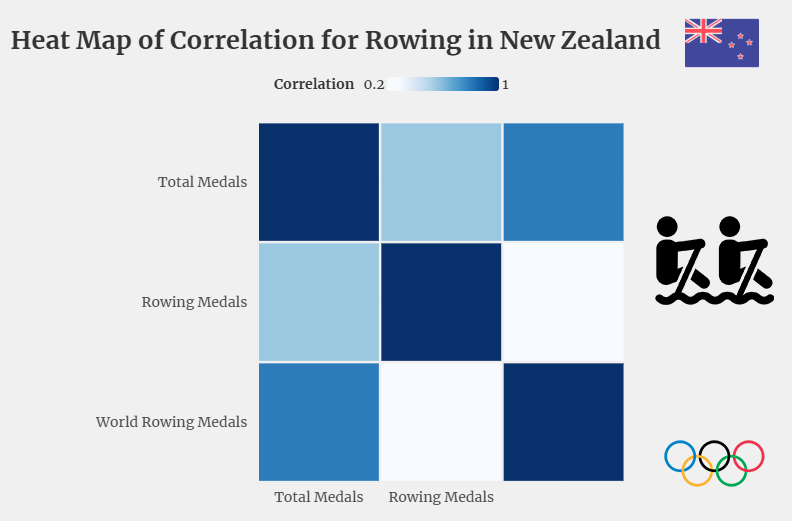
\includegraphics[width=\textwidth]{img/New Zealand.png}
		\caption{Heatmap of Correlation for Rowing in New Zealand}\label{subfig:3}
	\end{subfigure}
	\caption{Heatmap of Correlation}\label{fig:subfigures}
\end{figure}

We found that although China has a significant advantage in table tennis, the relationship between the development of the event and China's total medal count is relatively weak. This suggests that China's overall athletic adeptness is \textbf{stable} and less influenced by a single dominant event.

Additionally, Jamaica's total medal count shows a strong positive correlation with its performance in athletics, indicating the country's heavy reliance on athletics competitions. Since athletics is a well-established and stable event with minimal fluctuations in the number of events held each year, the relationship between the number of events and Jamaica's total medal count is \textbf{relatively weak}. 

New Zealand also has a high dependency on rowing, with a substantial portion of its medals coming from this event. However, unlike Jamaica, rowing is not as established as athletics, and the number of competitions fluctuates from year to year. As a result, New Zealand's overall medal count is highly \textbf{dependent} on the rise and fall of rowing's prominence.
\subsection{Model Performances}

We calculated four evaluation metrics: Mean Squared Error (\textbf{MSE}), Root Mean Squared Error (\textbf{RMSE}), Mean Absolute Error (\textbf{MAE}), and the Coefficient of Determination (\(\mathbf{R}^2\)).

Among these, smaller values for the first three metrics and a larger value for R² indicate better model performance.

% \usepackage{longtable}

\begin{longtable}{l|l|l|l|l} 
	\caption{Model Performances(LightGBM)}\\ 
	\hline
	\multicolumn{1}{c|}{\textbf{Model}} & \multicolumn{1}{c|}{\textbf{MSE}} & \multicolumn{1}{c|}{\textbf{RMSE}} & \multicolumn{1}{c|}{\textbf{MAE}} & \multicolumn{1}{c}{\(\mathbf{R}^2\)}  \endfirsthead 
	\hline
	Gold Prediction                     & 0.0235                            & 0.180                              & 0.030                             & 0.890                              \\ 
	\hline
	Silver Prediction                   & 0.0239                            & 0.185                              & 0.033                             & 0.825                              \\ 
	\hline
	Bronze Prediction                   & 0.0231                            & 0.187                              & 0.034                             & 0.806                              \\
	\hline
\end{longtable}


%雷达图
\begin{figure}[H]
	\centering
	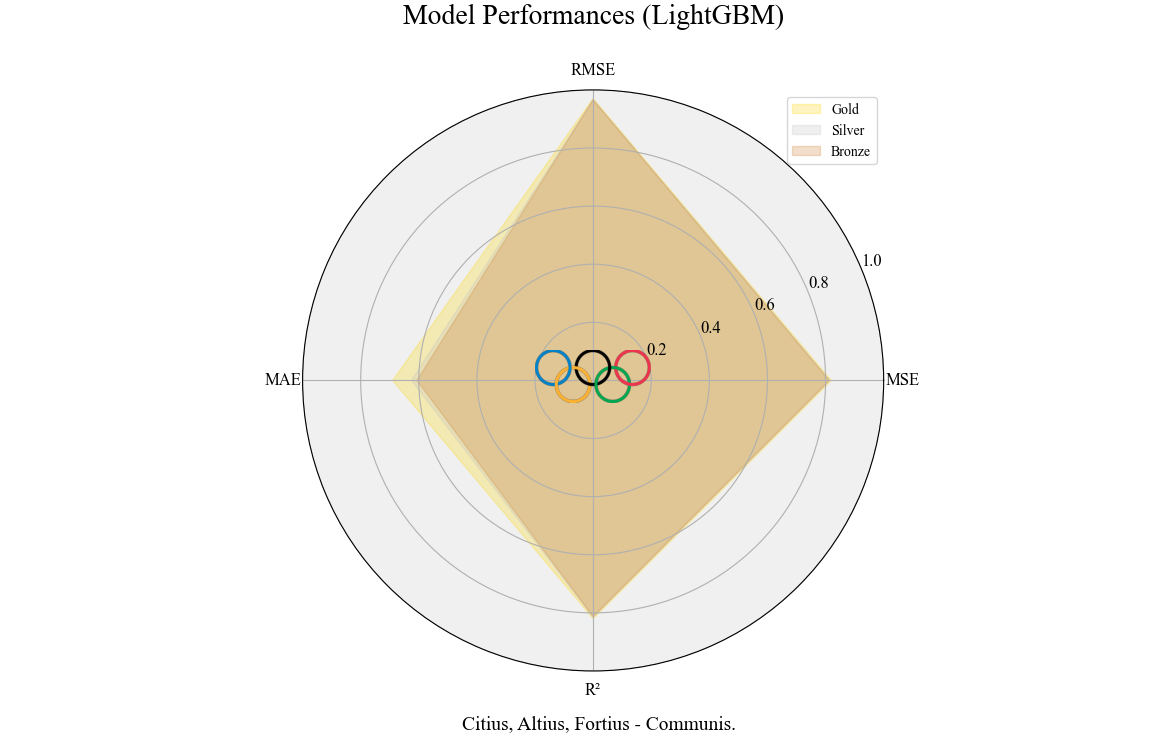
\includegraphics[width=8cm]{img/Performance.png}
	\caption{Model Performance Radar Chart}
	\label{fig:aa}
\end{figure}


It can be observed that the evaluation metrics for the prediction of the 3 types of medals show good performance with relatively small differences. 

A comparison reveals that the model's prediction accuracy for gold medals is relatively higher, with the highest \(\mathbf{R}^2\) and the lowest Root Mean Squared Error (RMSE) and Mean Absolute Error (MAE).





%引用图像示例Figure \ref{fig:subfigures}
%Figure \ref{fig:subfigures} gives an example of subfigures. Figure \ref{subfig:left} is on the left, and Figure \ref{subfig:right} is on the right.



\section{Task2:Great Coach Effect}
\subsection{Verification of the Great Coach Effect}
The Great Coach effect can cause significant differences in the performance of relevant countries in corresponding events. To collect evidence of changes caused by this effect, we use a \textbf{Bayesian Changepoint Detection (BEAST)} model.

The BEAST model uses Bayesian inference to calculate the posterior probabilities of changes occurring at different time points, determining which time points are potential change points.

In the time series dataset \(X = (x_1, x_2, x_3, \ldots, x_T)\), we identify the set of change points \(C = \{c_1, c_2, \ldots, c_K\}\), where each \(c_k\) represents a change point.

Using Bayes' theorem, we can compute the \textbf{posterior probability} for each possible change point $c_k$:

\begin{equation}
	P(c_k \mid X) = \frac{P(X \mid c_k) P(c_k)}{P(X)}
\end{equation}

In this case, \( P(X|c_k) \) represents the likelihood of the data at the change point \( c_k \), \( P(c_k) \) is the prior probability, and \( P(X) \) is the marginal likelihood of the data.

By calculating the posterior probability for each change point, we can identify the moments when significant changes occurred in the data.

Thus, we simply need to extract the historical award data for the relevant countries and events from the dataset and perform Bayesian Changepoint Detection.

This allows us to determine how much influence these great coaches had on the medal counts achieved by these countries in the relevant events during the periods when Lang Ping coached the Chinese and U.S. volleyball teams, and when Bela Karolyi coached the Romanian and U.S. women's gymnastics teams.

Since the value of gold, silver, and bronze medals is not the same, we standardized the data by assigning weights to the medals. The final medal count in the dataset is calculated as follows: 



%公式 未知




Taking Lang Ping's leadership of the Chinese and U.S. volleyball teams as an example, we extracted the data for Chinese and U.S. volleyball from the original medal dataset. Through Bayesian Changepoint Detection, we found that the period when Lang Ping changed coaching countries coincided with a significant change in the dataset, as shown in the figure below:



%5.1 排球
\begin{figure}[H]
	\centering
	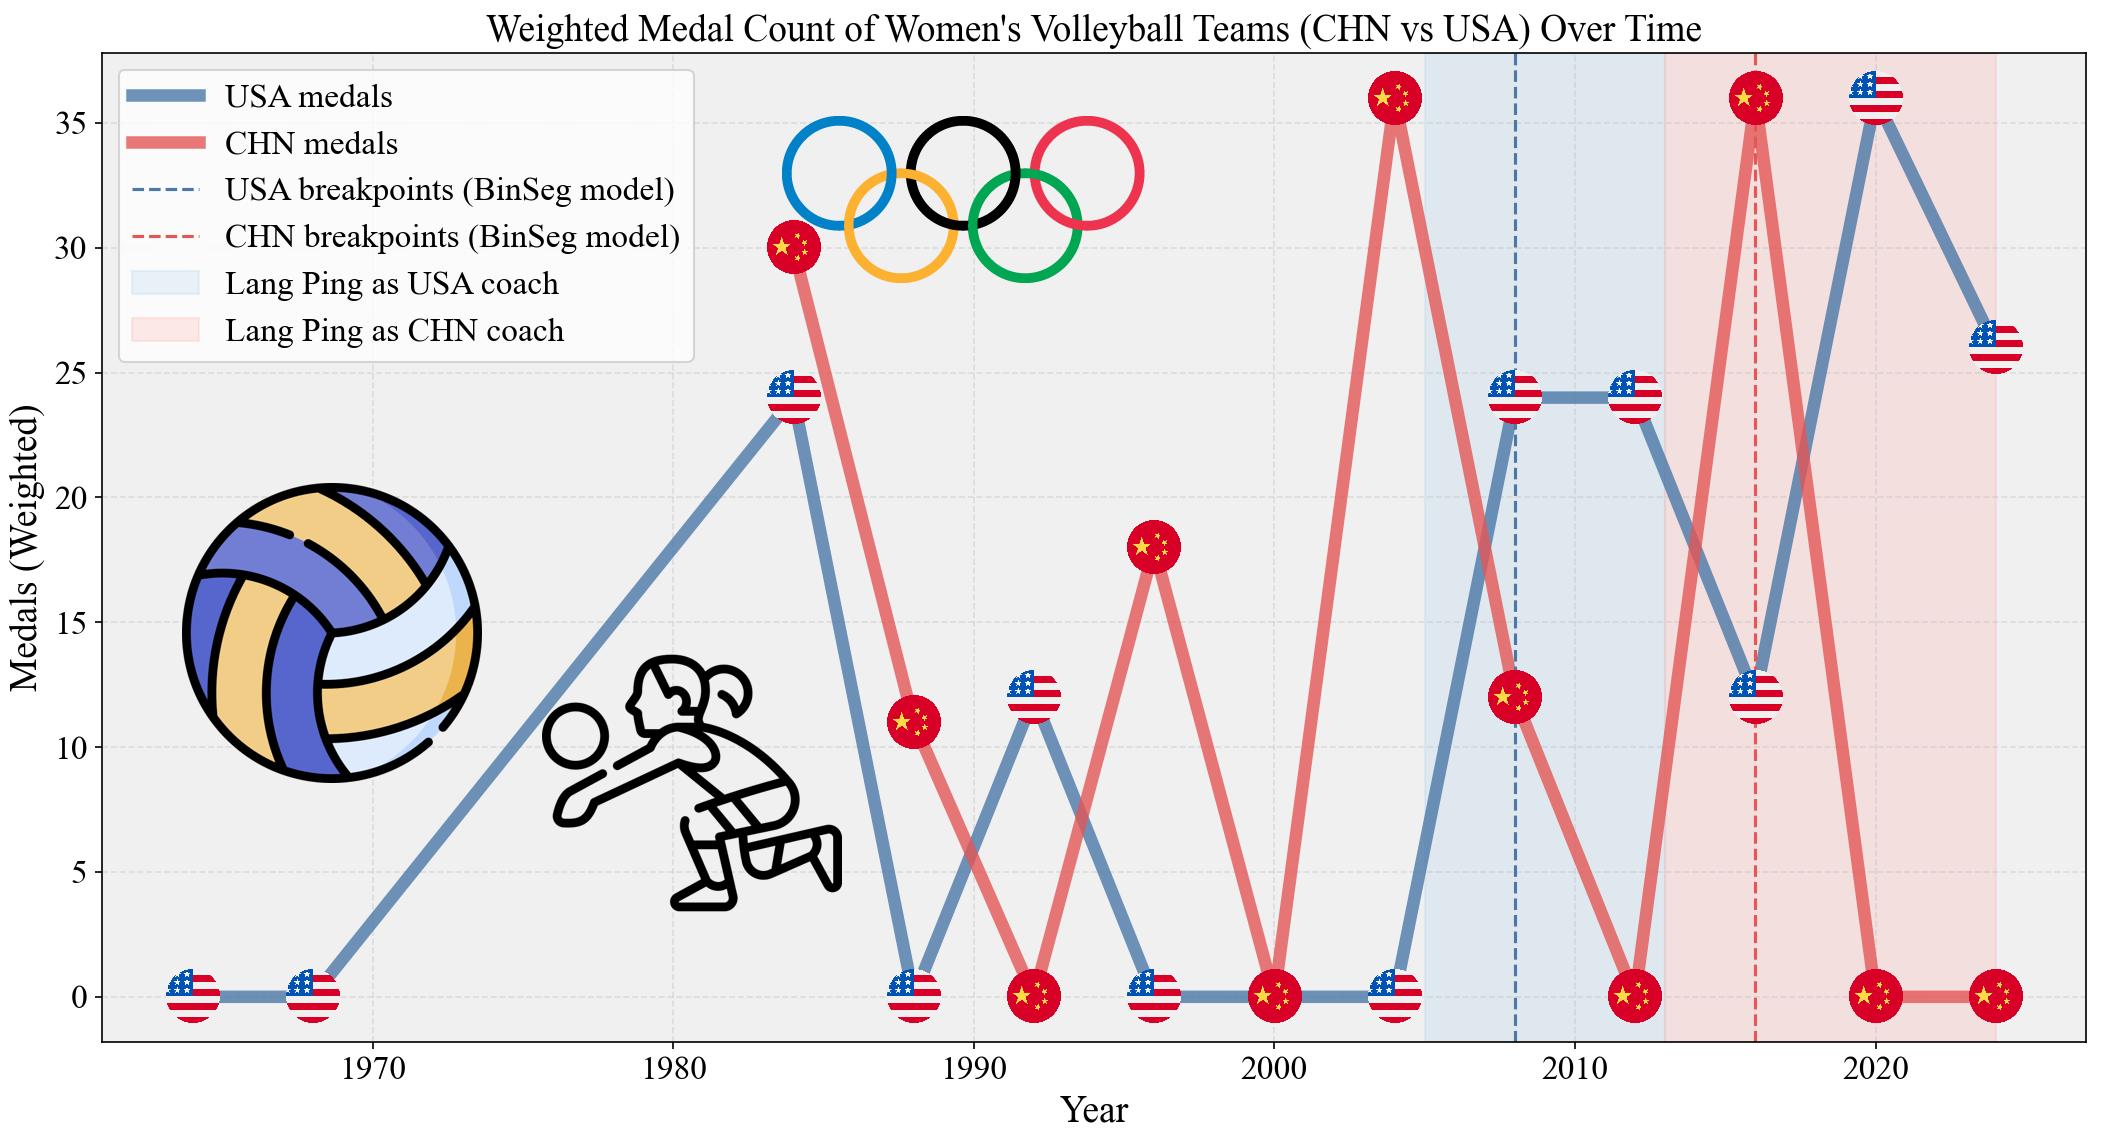
\includegraphics[width=12cm]{img/Volleyball.png}
	\caption{Medal Count of Women's Volleyball Teams(CHN vs USA) Over Time}
	\label{fig:aa}
\end{figure}
Clearly, after Lang Ping began coaching the U.S. team in 2005, the U.S. volleyball team showed remarkable improvement in the next Olympic Games, while the Chinese team experienced significant regression. However, after Lang Ping returned to coach China in 2013, the Chinese team quickly rose from the trough and regained their peak performance, while the U.S. team showed a decline.

Between 2016 and 2020, the Chinese team underwent a period of stagnation due to the retirement of key players and the lack of a strong new generation.

Similarly, Bela Karolyi's coaching of the Romanian and U.S. women's gymnastics teams shows significant changes, with similar patterns to Lang Ping's coaching history. In addition, we also studied other similar cases. Therefore, we can conclude that the great coach effect has a significant impact on a country's medal count in the corresponding event.


\subsection{Countries Recommended for Hiring Coaches}
After confirming the significant impact of the great coach on the medal count, we began to analyze which events a country should consider investing in great coaches. For this, we use the \textbf{CUSUM} algorithm.

The CUSUM method detects deviations in a data sequence by calculating the cumulative sum, which is the running total of the deviation between each data point and the expected or baseline value. It is effective at detecting small changes in the mean and has been widely used in quality control, process monitoring, and other fields.

We select the forward CUSUM to detect trends in the medal count of a particular country's sports event. If the curve shows a prolonged downward trend, it indicates a significant regression in that event, suggesting the need for a coach change.

\begin{equation}
	C_t^+ = \max(0, C_{t-1}^+ + (X_t - \mu - k))
\end{equation}

Here, $C_t^+ $represents the cumulative value of the forward CUSUM, $X_t$ is the t-th data point, $\mu$ is the expected or average value (target value), and $k$ is the threshold, indicating the allowable minimum deviation. Typically, a reasonable $k$ value is chosen, often a multiple of the process standard deviation.

If the curve shows a prolonged downward trend, it indicates that the event has significant regression, suggesting the need for a coach. The results obtained are as follows:



%三个国家某项目衰弱 需要教练图
\begin{figure}[H]
	\centering
	\begin{subfigure}[b]{.32\textwidth}
		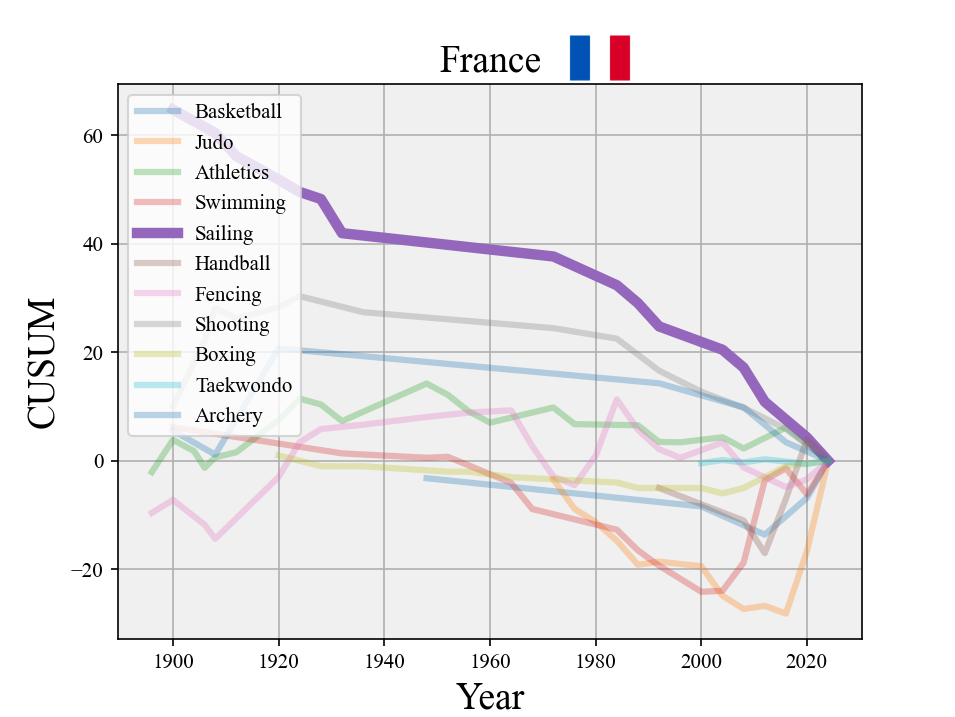
\includegraphics[width=\textwidth]{img/Decline1.png}
		\caption{France}\label{subfig:1}
	\end{subfigure}
	\hfill 
	\begin{subfigure}[b]{.32\textwidth}
		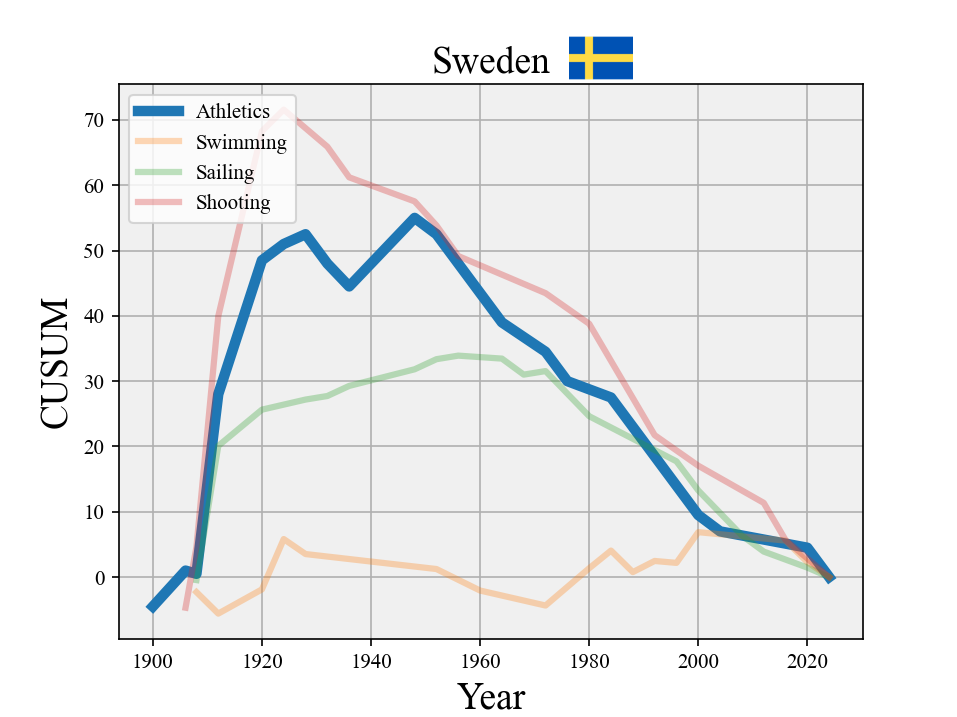
\includegraphics[width=\textwidth]{img/Decline2.png}
		\caption{Sweden}\label{subfig:2}
	\end{subfigure}
	\hfill 
	\begin{subfigure}[b]{.32\textwidth}
		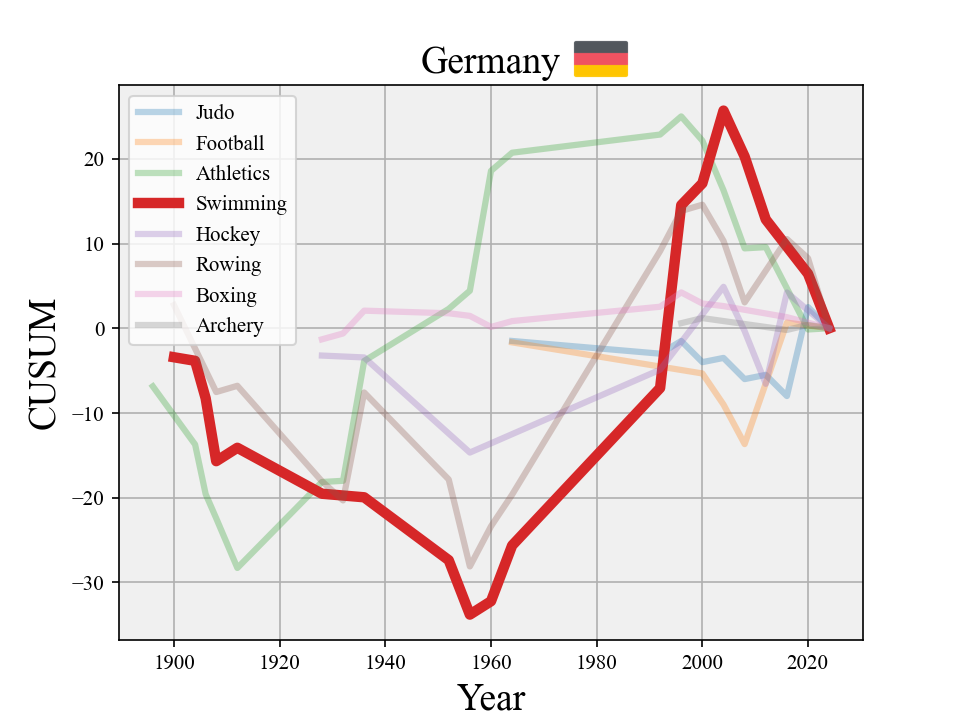
\includegraphics[width=\textwidth]{img/Decline3.png}
		\caption{Germany}\label{subfig:3}
	\end{subfigure}
	\caption{Three images}\label{fig:subfigures}
\end{figure}

We observe that sailing was a dominant event for France when the earliest Olympic Games were held. Although it did not remain as developed in the subsequent years, it still maintained relatively stable results from the 1930s to the 1970s. However, after the 1970s, there was a clear downward trend, which suggests the need to hire a coach.

Sweden's dominance in athletics and shooting during the 1920s to 1950s showed significant advantages, but both events have experienced a substantial decline over time, possibly due to a decrease in the nation's emphasis on events competitions. Therefore, it is recommended to hire a coach.

Germany’s swimming did not show any notable advantage before the 1990s. However, at the beginning of the 21st century, it emerged as a new powerhorse. Yet, there are clear signs of decline in the 2010s to 2020s. To maintain swimming’s competitive edge, it would be beneficial to hire a coach.



\section{Task3:Other Original Insights}

\subsection{Gender Distribution}

We analyzed the gender ratio in the Olympics, focusing on two aspects: the male-to-female ratio of athletes participating in the Games and the male-to-female ratio of medal winners, as shown in the figure.

	%6.1 男女比例图
	\begin{figure}[H]
		\centering
		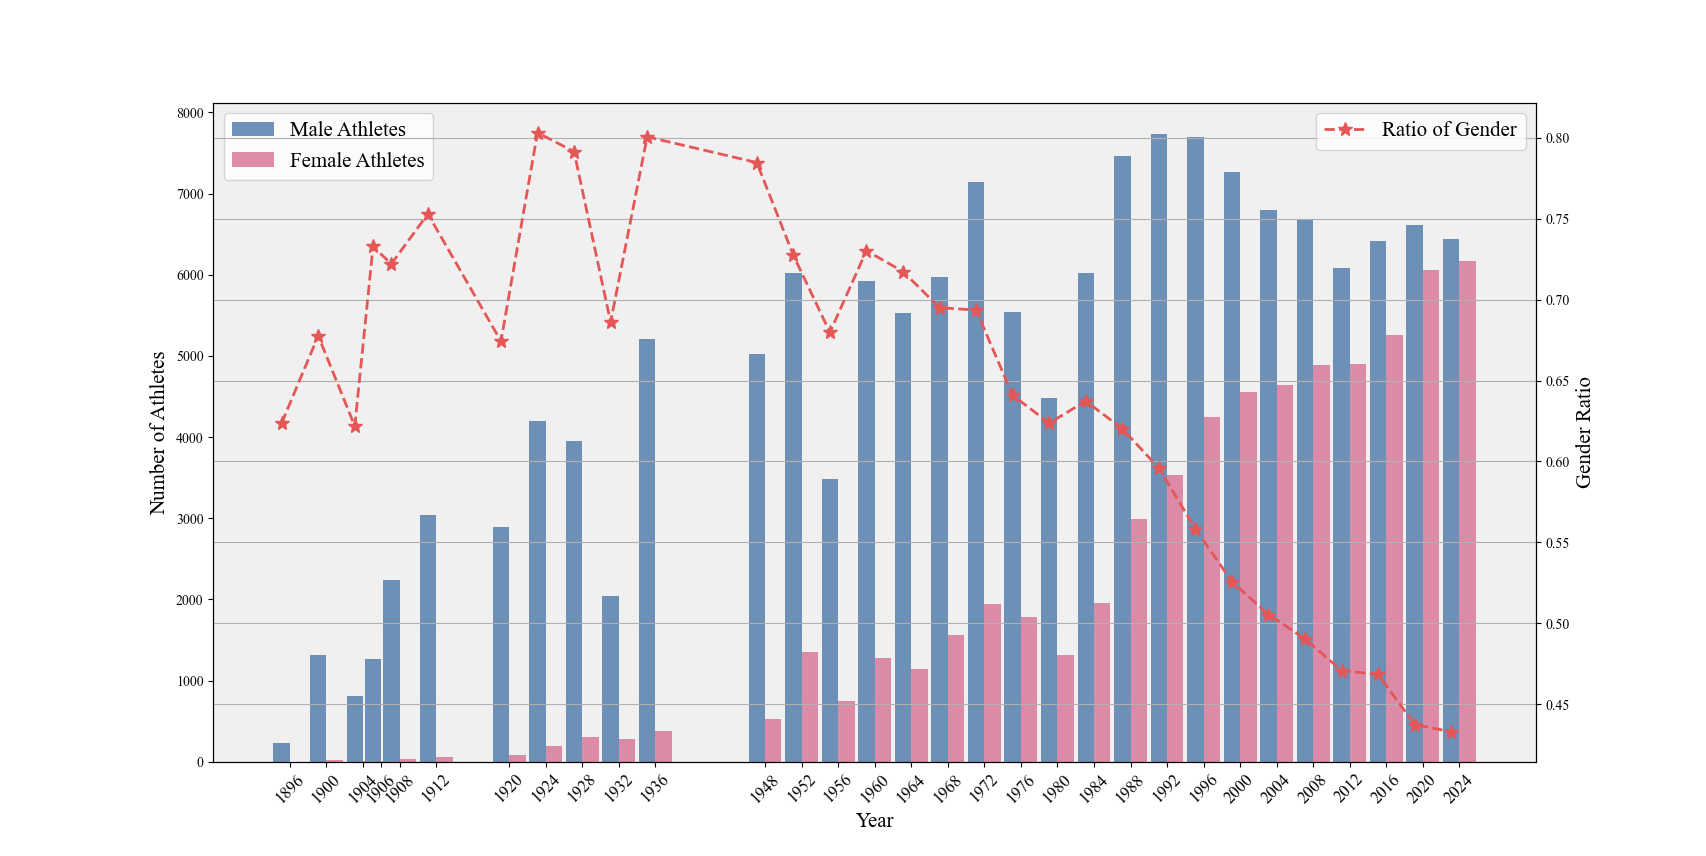
\includegraphics[width=12cm]{img/Gender with Award.png}
		\caption{Gender Distribution of Athletes(with Award)}
		\label{fig:aa}
	\end{figure}
	
	\begin{figure}[H]
		\centering
		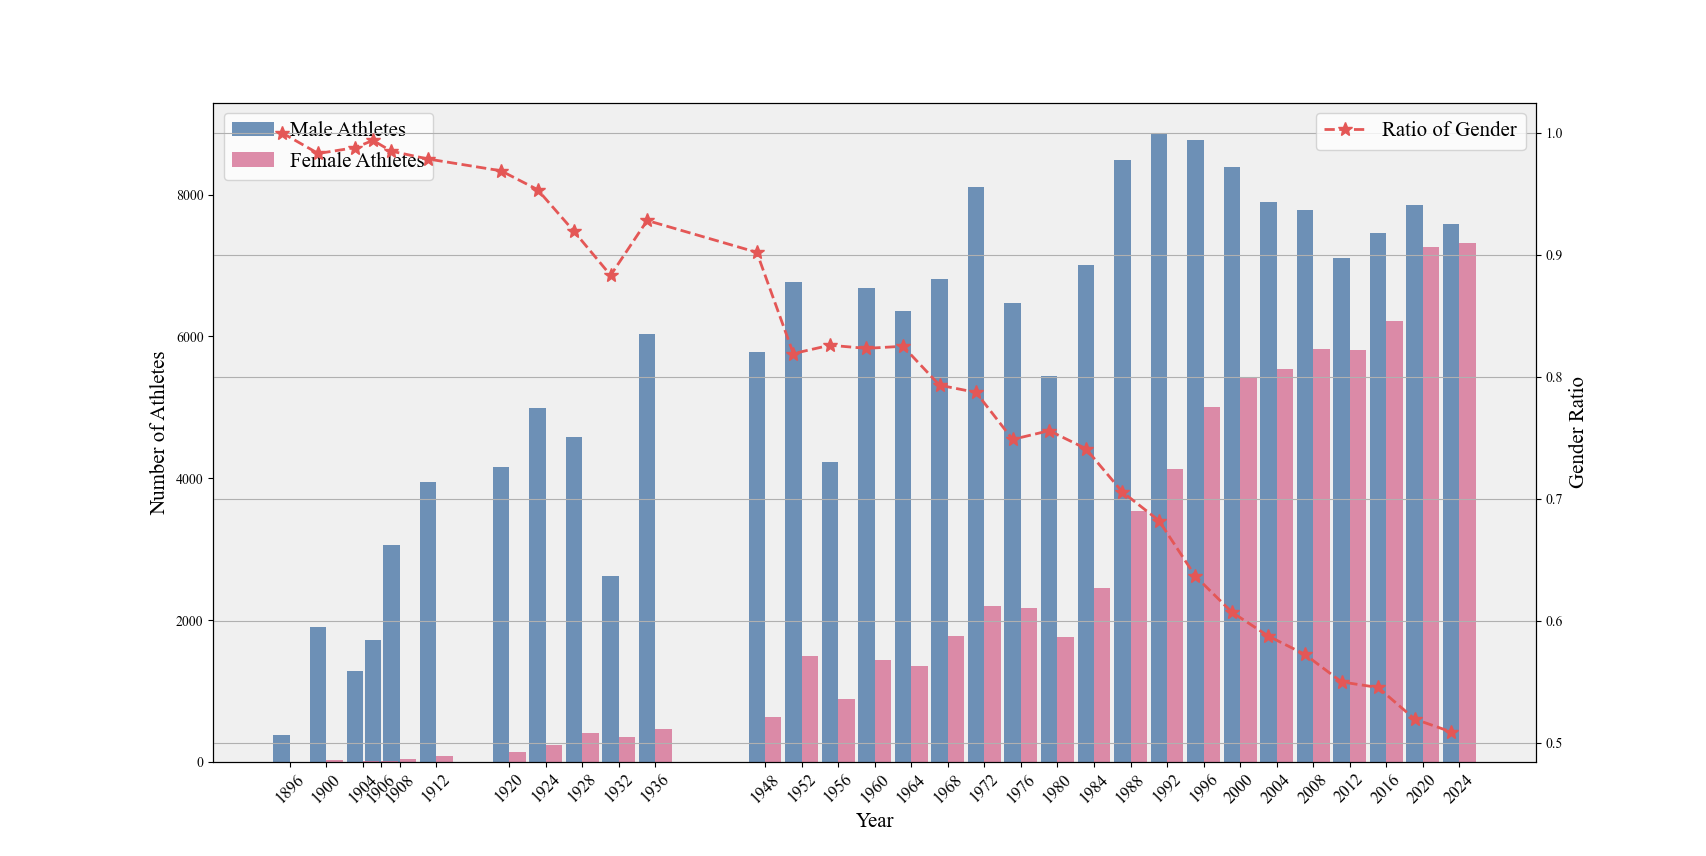
\includegraphics[width=12cm]{img/Gender.png}
		\caption{Gender Distribution of Athletes}
		\label{fig:aa}
	\end{figure}
	
Firstly, the \textbf{gender ratio} in the Olympics has become increasingly \textbf{balanced}, with the male-to-female ratio nearly equal, shifting from a male-dominated ratio to approximately 1:1. The number of female athletes has steadily increased over time, particularly in the late 20th and early 21st centuries, with a more pronounced growth trend.

This trend not only reflects the efforts of the International Olympic Committee and national events organizations to promote gender equality, including providing more opportunities for female athletes to participate and offering more events for women, but also signifies an increased societal awareness of gender equality, leading to more opportunities for women to engage in sports.

Moreover, the trends in the gender distribution of athletes (with awards) and the overall athlete distribution exhibit almost identical patterns of growth or decline.










%6.2
\subsection{Dominant Sports}

In analyzing the national strengths in specific events, we found that certain countries have a \textbf{dominant advantage}, even to the point of forming a dominance, with their share of the total medal count reaching as high as \( 30\% \), \( 50\% \), or even over \textbf{\( 80\% \)}.



\begin{figure}[H]
	\centering
	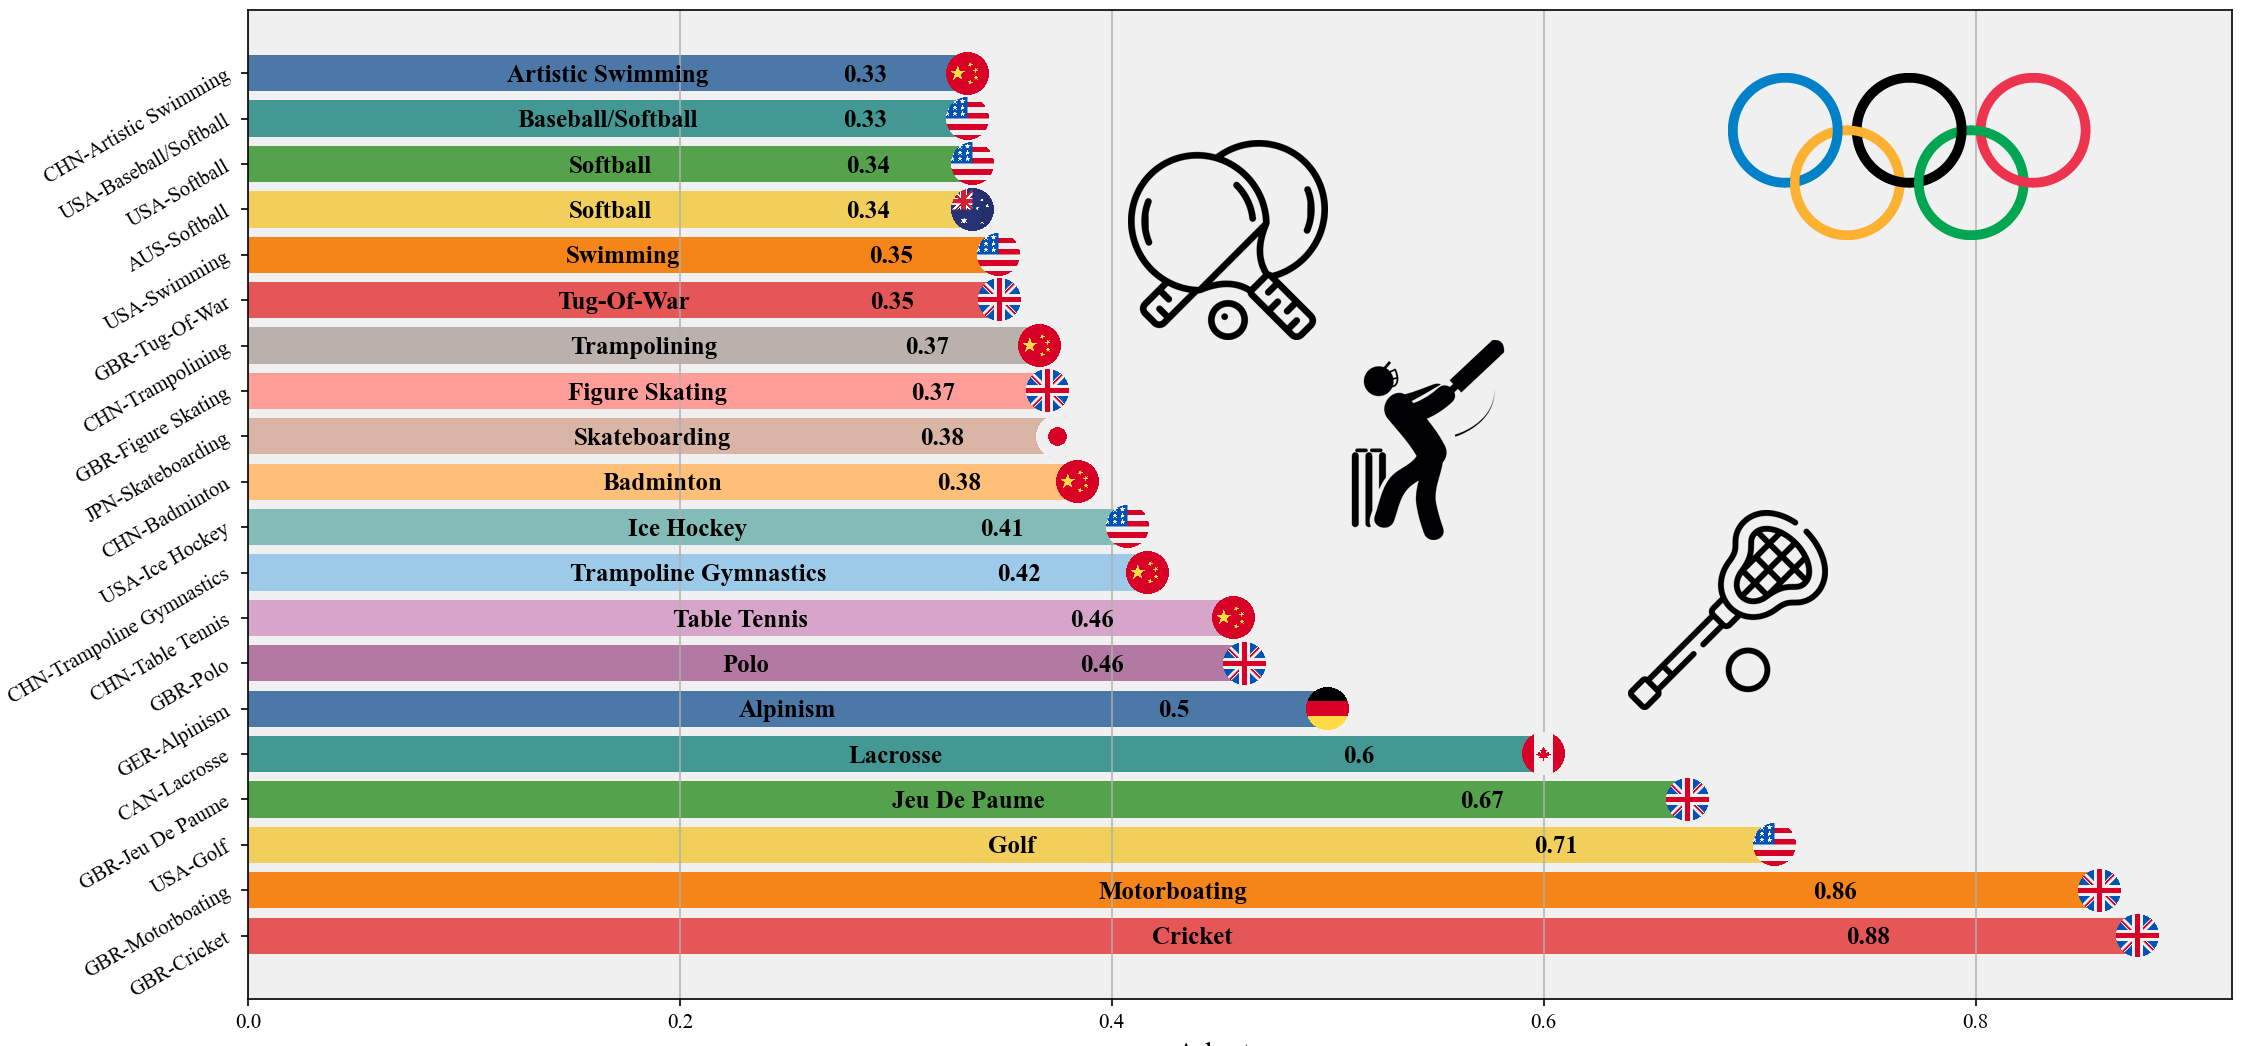
\includegraphics[width=16cm]{img/Monopolized Sports.png}
	\caption{Adeptness of Countries in Specific Event}
	\label{fig:aa}
\end{figure}

As shown in the figure, the United Kingdom holds an astonishing dominance in Motorboating and Cricket. Since Motorboating has only appeared twice in the Olympics and Cricket is a newly added event in the 2028 Olympics, these events are not highly regarded by other countries, except for the UK, which has a natural advantage in these traditional sports.

Therefore, we suggest that national Olympic committees consider investing in such events if they aim to win more medals.


Among the events commonly featured in recent Olympics, table tennis serves as a very typical example. China, with a remarkable \( 46\% \) share of table tennis medals, holds a monopoly advantage in this event. This is due to the development of a professional and efficient events system, strongly supported by the Chinese government.

Based on the previously confirmed \textbf{great coach effect}, if other countries wish to enhance their capabilities in these events and win more medals, they may consider hiring coaches from these dominant countries.



%6.3
\subsection{Global Geopolitics}
As of now, the Olympics has been held 33 times, spanning from 1896 to 2024, covering nearly 130 years. Thus, the Olympics has witnessed the dramatic shifts in global geopolitics throughout the 20th century. We created a stacked area chart based on each country's share of the total medals, offering a glimpse into the significant impact of world affairs on Olympic results.

%6.3 花里胡哨图
\begin{figure}[H]
	\centering
	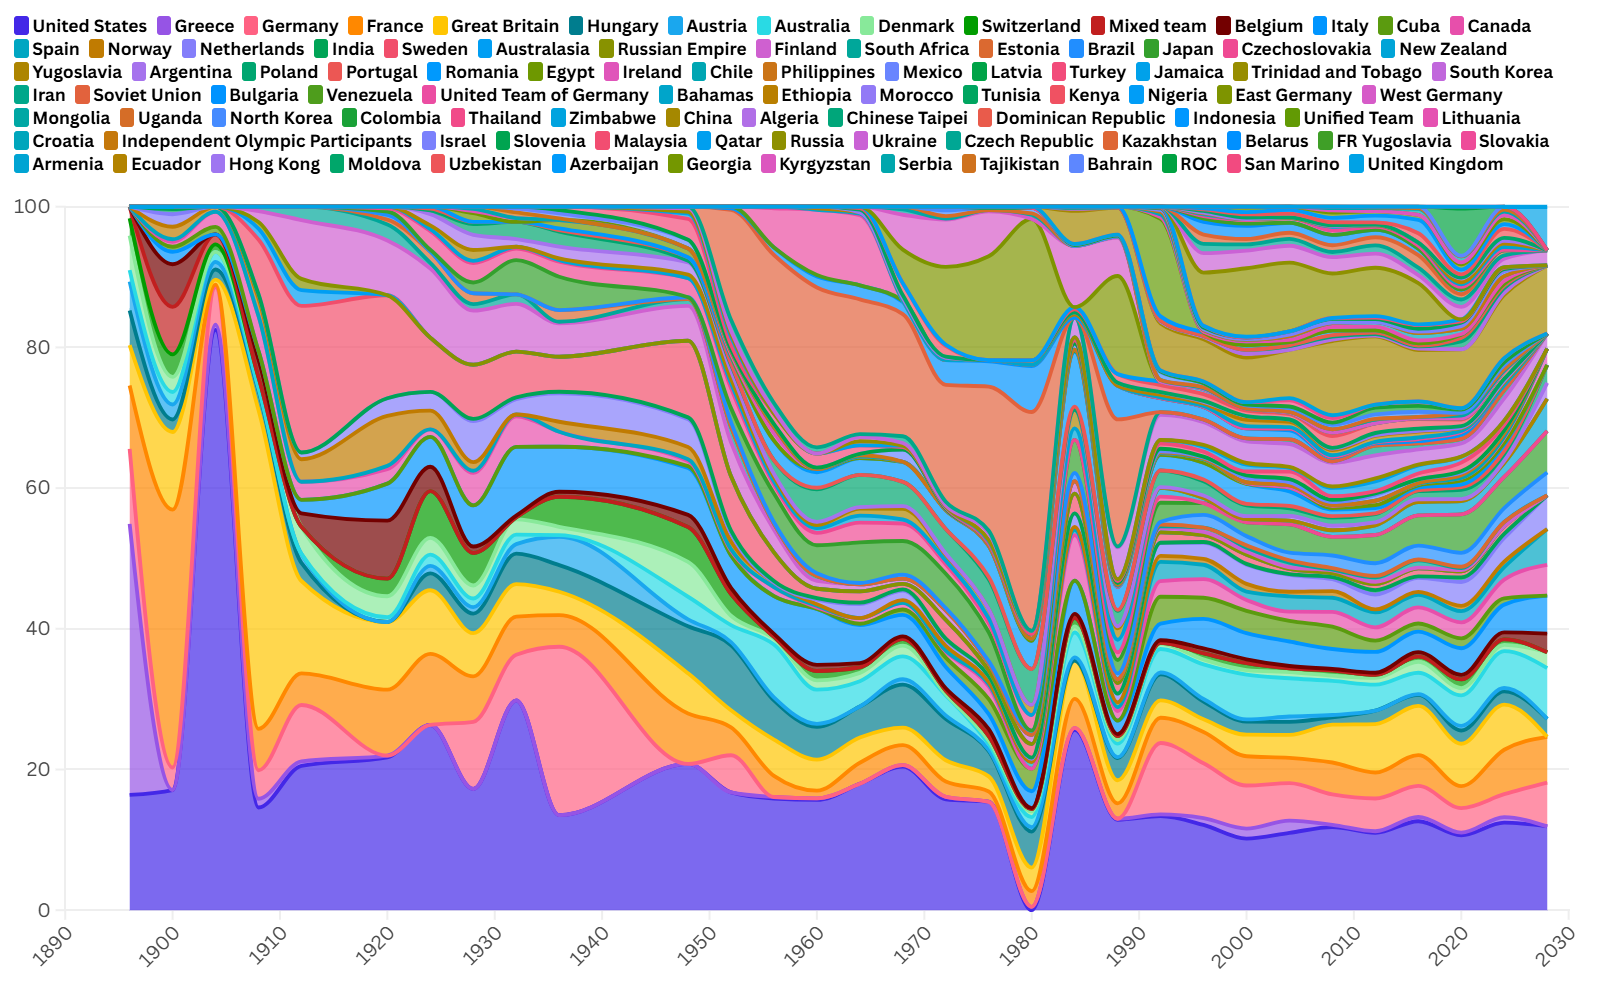
\includegraphics[width=16cm]{img/3.3-1.png}
	\caption{Trend of Medal Proportions by Country Annually}
	\label{fig:aa}
\end{figure}

From the chart, we can observe four notable anomalies in the medal distribution: in 1904, 1980, 1984, and 1992.

The 1904 Olympics, held in St. Louis, Missouri, USA, lasted five and a half months. Due to the long travel distance and the absence of U.S. President Theodore Roosevelt and IOC President Pierre de Coubertin at the opening and closing ceremonies, only 12 countries participated, marking the lowest number of participating countries in Olympic history. The U.S. dominated the medal count with a significant lead.

The 1980 Olympics, held in Moscow, saw a boycott led by the United States in response to the Soviet invasion of Afghanistan in 1979. Around 65 countries, mostly from the Western bloc, refrained from sending athletes. As a result, the participating nations were primarily from the socialist camp, especially the Soviet Union and Eastern European countries, with the Soviet Union winning the most medals.

Similarly, the 1984 Los Angeles Olympics was also politically influenced. Following the 1980 boycott, the Soviet Union and other Eastern Bloc countries decided to boycott the 1984 Games in retaliation. The 1984 Olympics marked a significant turning point in Olympic history, showcasing the U.S.'s strong capabilities in organizing the event and symbolizing the beginning of the commercialization of the Games.

The 1992 Barcelona Olympics was a pivotal event, both as a major competition in the post-Cold War era and a reflection of significant global political changes. While political issues in certain countries and regions may still cause fluctuations in participation, the confrontational situation of the Cold War no longer had a frequent impact on the hosting and participation in the Games.

From the chart, it is evident that after the 1992 Olympics, the distribution of Olympic medals stabilized, and the development of the Olympics became more consistent.



\section{Sensitivity Analysis}

\textbf{Sensitivity Analysis} is used to evaluate the sensitivity of model outputs to changes in input features. Through this analysis, we can quantify the dependency of final prediction results prediction outcomes on specific data features, such as the adeptness of a particular country in a specific event or the previous award probability of an athlete.

LightGBM comes with a feature importance function that identifies the features with the greatest impact on the model’s predictions. By using \textbf{\textit{plot\_importance()}} function, we can visualize the importance of each feature.


\begin{figure}[H]
	\centering
	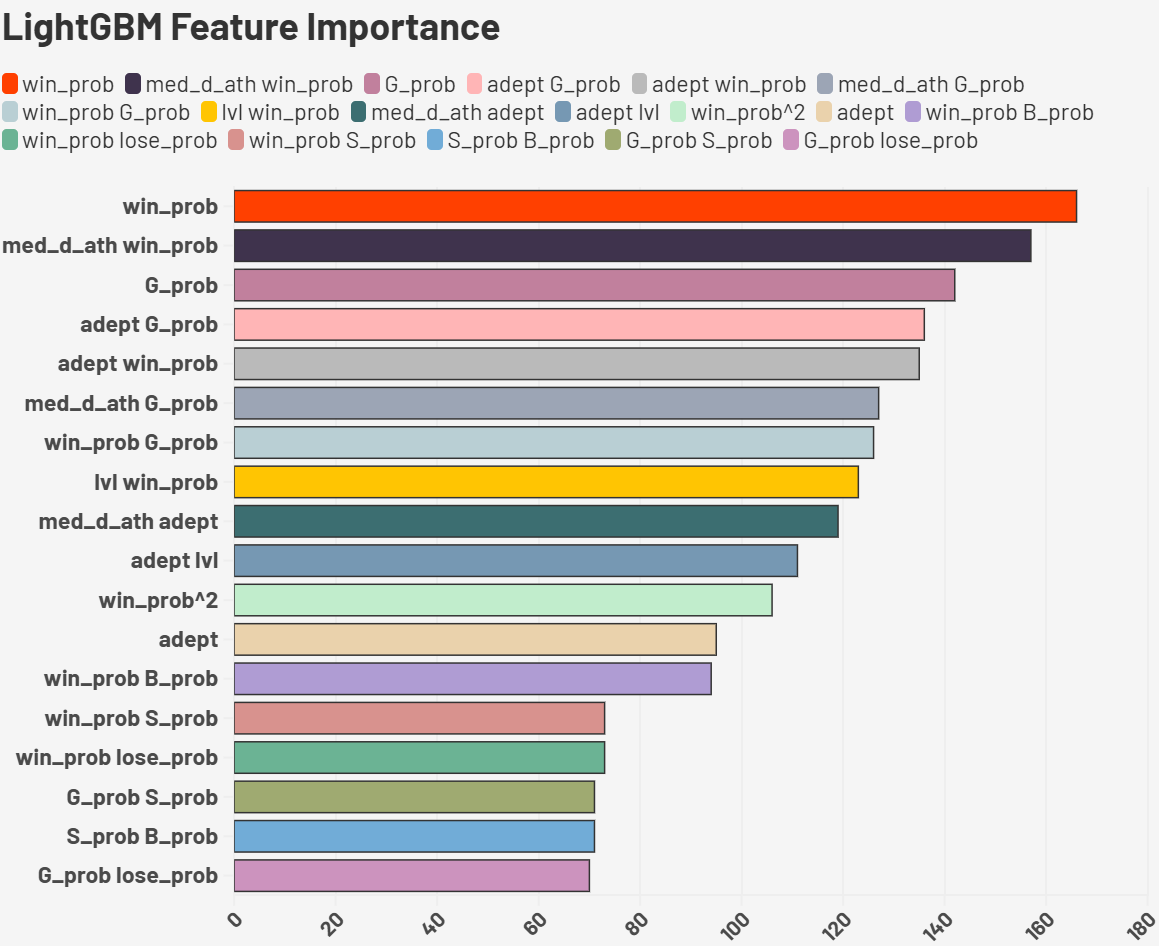
\includegraphics[width=13cm]{img/Sensitive Analysis 1.png}
	\caption{LightGBM Feature Importance}
	\label{fig:aa}
\end{figure}

The above figure shows the feature importance distribution for the gold medal prediction model. Since we generated PolynomialFeatures during training, the features observed here are the products of several individual features.

From the figure, we can see that the probability of an athlete winning a medal in the past, as well as the degree of a country's advantage in a specific event, have the greatest influence on the final prediction results. Additionally, the athlete’s past medal-winning probability also has a significant impact on the prediction.

Furthermore, we can use Shapley value analysis to assess the model's sensitivity. \textbf{SHAP} (\textbf{SH}apley \textbf{A}dditive ex\textbf{P}lanations) is a game theory-based model explanation method used to interpret machine learning model predictions. It assigns each feature a contribution to the model's prediction, helping us understand the importance and influence of each feature in the given prediction result.The formula for Shapley value is as follows:


\begin{equation}
	\phi_i(f) = \sum_{S \subseteq N \setminus \{i\}} \frac{|S|!(|N|-|S|-1)!}{|N|!} [ f(S \cup \{i\}) - f(S)]
\end{equation}


\textbf{\(\phi_i(f)\)} is the Shapley value of feature \textbf{\(x_i\).\(S\)} is a subset of features, and \(S \subseteq N \setminus \{i\}\) indicates that subset \textbf{\(S\)} contains all features except for \textbf{\(x_i\).\(f(S)\)} is the model's prediction on the feature subset \textbf{\(S\)}.
\textbf{\(f(S \cup \{i\})\)} is the model's prediction on the subset \textbf{\(S\)} and feature \textbf{\(x_i\)}.

\textbf{\(|S|!\) }and \textbf{\((|N|-|S|-1)!\)} are the \textbf{combinatorial coefficients} of the Shapley value, used to weigh the importance of each feature in different feature subsets.
\textbf{\(|N|!\)} is the total number of permutations of all features in the feature set \textbf{\(N\)}, ensuring the average effect across all permutations.

Below are the SHAP Summary Plots for the gold, silver, and bronze medal prediction models.


%三个奖牌的图像
\begin{figure}[H]
	\centering
	\begin{subfigure}[b]{.32\textwidth}
		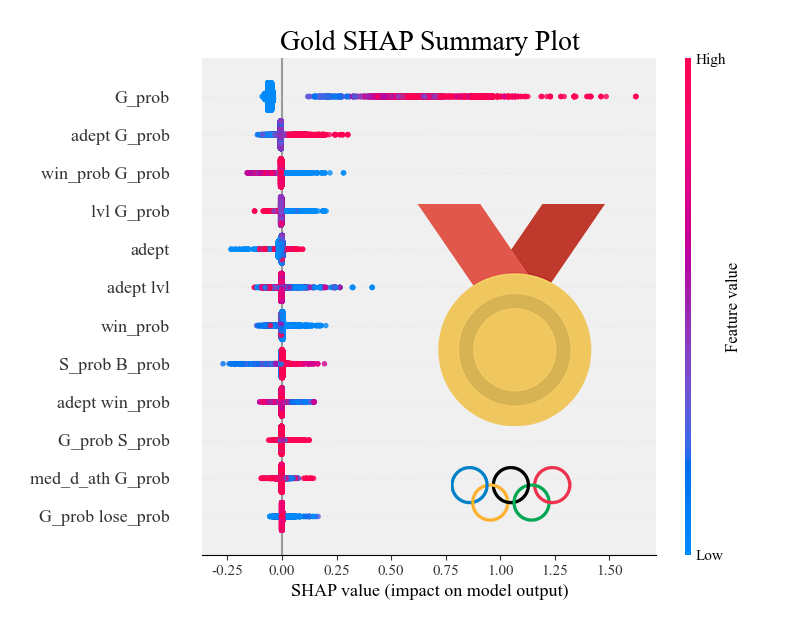
\includegraphics[width=\textwidth]{img/shap1.png}
		\caption{Gold SHAP Summary Plot}\label{subfig:1}
	\end{subfigure}
	\hfill 
	\begin{subfigure}[b]{.32\textwidth}
		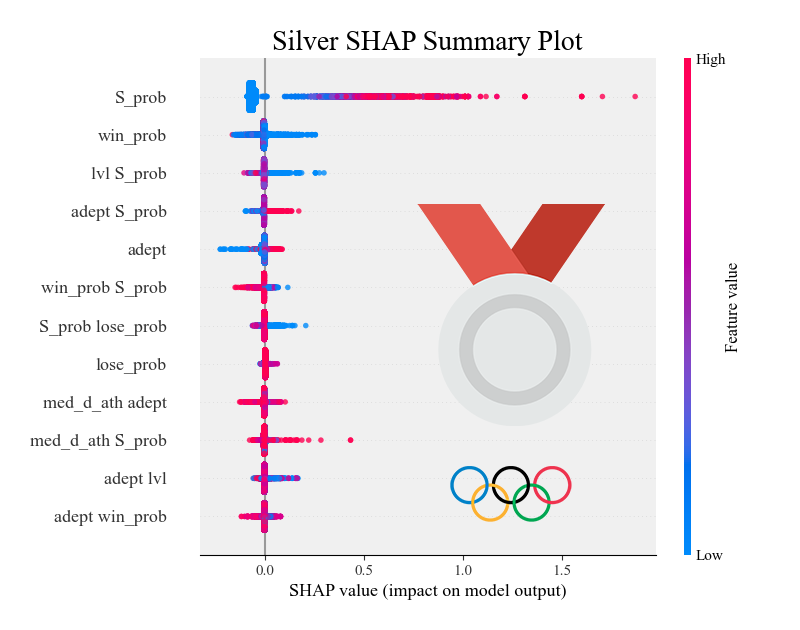
\includegraphics[width=\textwidth]{img/shap2.png}
		\caption{Silver SHAP Summary Plot}\label{subfig:2}
	\end{subfigure}
	\hfill 
	\begin{subfigure}[b]{.32\textwidth}
		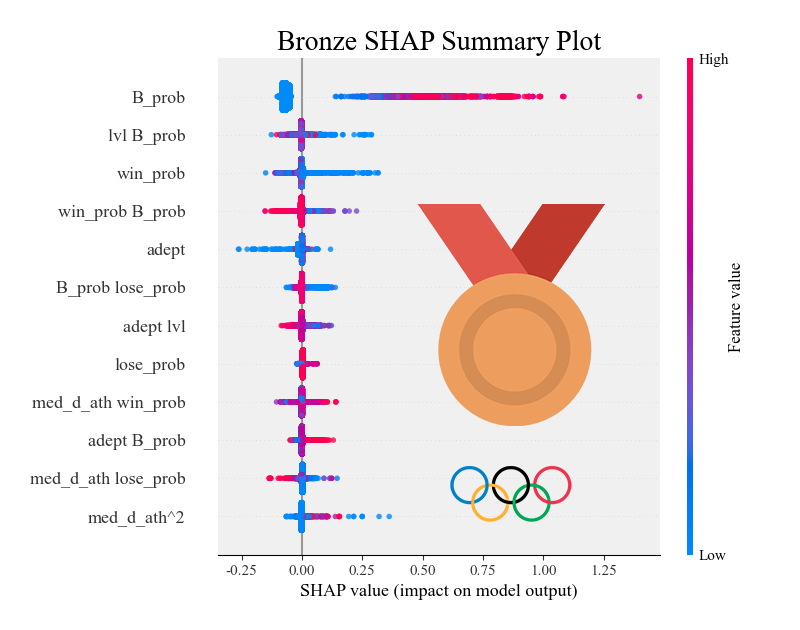
\includegraphics[width=\textwidth]{img/shap3.png}
		\caption{Bronze SHAP Summary Plot}\label{subfig:3}
	\end{subfigure}
	\caption{SHAP Summary Plots}\label{fig:subfigures}
\end{figure}
From the figures, we can see that the SHAP algorithm amplifies the prior probability of winning a particular medal. In other words, athletes who have previously won gold medals have a higher probability of winning gold again if they continue to compete, and the same holds true for silver and bronze medalists. This differs somewhat from the results obtained through LightGBM's self-analysis; however, both analysis methods assign relatively high weights to Adeptness, Level, and Win Probability.

\section{Model Evaluation}
\subsection{Strengths}
1. For medal prediction, we performed complex feature engineering and data mining, resulting in a large dataset. LightGBM is highly efficient in training, with fast processing speeds, low memory consumption, and support for parallel and distributed training, making it well-suited for handling large-scale data, aligning well with our dataset.

2. The model demonstrates high prediction accuracy, superior performance, and the predicted results align closely with expectations from previous years. Additionally, the predictions are consistent with common knowledge and offer high interpretability.

3. The model takes into account various indirect factors, such as a country's ranking, the types of sports a country excels in, whether the host is the organizer, athletes' prior competition status, and more. These factors enable the model to consider a broader range of real-world conditions, making it more aligned with actual data.

4. The Bayesian Change Point Detection used in Task 2 accurately reflects the change points in time-series data. Our tests showed that the change points in the performance of China and the United States women's volleyball teams coincided with the coaching periods of Lang Ping, demonstrating the model's accuracy.
\subsection{Weaknesses}
1. Since the training data includes a large amount of historical data (spanning over 50 years), the prediction results are susceptible to the influence of historical data, leading to potential errors.

 	
 	

\section{Conclusion}
\begin{itemize}
		\item \textbf{Task1}
		

We applied data preprocessing and feature engineering, using the \textbf{KMeans++} clustering algorithm to rank countries based on various features, including proficiency in different sports, host nation advantages, and athlete performance levels.

The \textbf{LightGBM} regression model predicted the medal count for each country in the 2028 Olympics. Our analysis indicated that the United States is likely to progress, while France may decline, largely due to the home-field advantage. Countries such as Australia and Japan are expected to see an increase, while Italy and South Korea may experience a decrease.

China's medal count is projected to remain stable. For nations without prior medals, we identified \textbf{Sierra Leone}, \textbf{Antigua and Barbuda}, and \textbf{Papua New Guinea} as those with the highest probability of winning their first medal in 2028. Correlation analysis revealed that countries with strong overall performance, like China, show minimal dependence on specific events, while smaller countries are more reliant on key events for their total medal count.
	

	\item \textbf{Task2}

We explored the great coach effect using the \textbf{Bayesian Changepoint Detection} model. We found a strong correlation between coaching tenures and significant changes in a country’s sports performance.
 
Additionally, the \textbf{CUSUM} algorithm helped identify weak events for several countries, such as France’s decline in sailing, Sweden’s waning dominance in athletics and shooting, and Germany’s emerging strength in swimming, which later showed signs of decline. Based on these findings, we recommend hiring specialized coaches to help maintain or regain competitive advantages in these events.
	\item \textbf{Task3}
	
The models and data from Task 1 and Task 2, we performed a \textbf{detailed analysis} of several key trends in the Olympics. We found that the athlete \textbf{gender ratio} has become more balanced over time, reflecting increasing gender equality.
 
Moreover, certain countries dominate \textbf{niche events}, such as the UK in cricket and Canada in lacrosse, which could offer opportunities for Olympic committees to enhance their medal prospects by investing in these specialized events. Lastly, our analysis of medal distribution changes over time revealed significant anomalies in 1904, 1980, 1984, and 1992, reflecting the Olympics' evolution and \textbf{geopolitical shifts}, particularly during the Cold War. These anomalies provide insights into broader global political and economic changes.
\end{itemize}


% 参考文献,此处以 MLA 引用格式为例
\begin{thebibliography}{99}
\bibitem{1}R. Prescott Adams, D.J.C. MacKay Bayesian Online Changepoint Detection 
\emph{Technical Report}, (2007)
\bibitem{2}G. Ke, Q. Meng, T. Finley, T. Wang, W. Chen, W. Ma, et al.
LightGBM: a highly efficient gradient boosting decision tree
\emph{Proceedings of the 31st International Conference on Neural Information Processing Systems}. (2017), pp. 3149-3157
\bibitem{3}Arthur, D., \& Vassilvitskii, S. . K-means++: The advantages of careful seeding.
\emph{Proceedings of the Annuual ACM-SIAM Symposium on Discrete Algorithms}.(2007)8, 1027-1035. 10.1145/1283383.1283494.
\bibitem{4}Mosca, Edoardo, Ferenc, Szigeti, Stella, et al.
TragianniSHAP-based explanation methods: A review for NLP interpretability
\emph{In Proceedings of the 29th International Conference on Computational Linguistics}.2022

\bibitem{5}Seiler S. Evaluating the (your country here) Olympic medal count.
\emph{Int J Sport Physiol Perform.}.2013;8:203–10.




\end{thebibliography}







% 以下为附录内容
% 如您的论文中不需要附录,请自行删除
\begin{subappendices}  % 附录环境


\section{Appendix A: Countries' Medal Count Prediction}

\begin{longtable}{|l|c|c|c|c|c|c|c|c|c|c|}
	\caption{Countries' Medal Count Prediction}\\
	\hline
	Country                                                        & \multicolumn{1}{l|}{\begin{tabular}[c]{@{}l@{}}G\_\\pes.\end{tabular}} & \multicolumn{1}{l|}{\begin{tabular}[c]{@{}l@{}}S\_\\pes.\end{tabular}} & \multicolumn{1}{l|}{\begin{tabular}[c]{@{}l@{}}B\_\\pes.\end{tabular}} & \multicolumn{1}{l|}{\begin{tabular}[c]{@{}l@{}}G\_\\opt.\end{tabular}} & \multicolumn{1}{l|}{\begin{tabular}[c]{@{}l@{}}S\_\\opt.\end{tabular}} & \multicolumn{1}{l|}{\begin{tabular}[c]{@{}l@{}}B\_\\opt.\end{tabular}} & \multicolumn{1}{l|}{Gold} & \multicolumn{1}{l|}{Silver} & \multicolumn{1}{l|}{Bronze} & \multicolumn{1}{l|}{Total}  \endfirsthead 
	\hline
	United States                                                  & 47                                                                     & 36                                                                     & 23                                                                     & 53                                                                     & 41                                                                     & 25                                                                     & 51                        & 40                          & 25                          & 117                         \\ 
	\hline
	China                                                          & 35                                                                     & 35                                                                     & 15                                                                     & 46                                                                     & 38                                                                     & 20                                                                     & 40                        & 36                          & 17                          & 95                          \\ 
	\hline
	Australia                                                      & 28                                                                     & 20                                                                     & 22                                                                     & 33                                                                     & 24                                                                     & 24                                                                     & 29                        & 22                          & 23                          & 71                          \\ 
	\hline
	France                                                         & 23                                                                     & 19                                                                     & 19                                                                     & 27                                                                     & 20                                                                     & 22                                                                     & 24                        & 19                          & 21                          & 64                          \\ 
	\hline
	Germany                                                        & 18                                                                     & 24                                                                     & 14                                                                     & 23                                                                     & 26                                                                     & 16                                                                     & 21                        & 25                          & 15                          & 61                          \\ 
	\hline
	United Kingdom                                                 & 20                                                                     & 19                                                                     & 14                                                                     & 26                                                                     & 24                                                                     & 15                                                                     & 25                        & 21                          & 15                          & 61                          \\ 
	\hline
	Japan                                                          & 16                                                                     & 25                                                                     & 14                                                                     & 19                                                                     & 27                                                                     & 16                                                                     & 17                        & 26                          & 16                          & 58                          \\ 
	\hline
	Italy                                                          & 15                                                                     & 20                                                                     & 15                                                                     & 17                                                                     & 20                                                                     & 22                                                                     & 16                        & 20                          & 16                          & 53                          \\ 
	\hline
	Spain                                                          & 21                                                                     & 10                                                                     & 13                                                                     & 30                                                                     & 12                                                                     & 14                                                                     & 25                        & 12                          & 13                          & 50                          \\ 
	\hline
	Netherlands                                                    & 24                                                                     & 6                                                                      & 13                                                                     & 29                                                                     & 9                                                                      & 15                                                                     & 26                        & 8                           & 15                          & 47                          \\ 
	\hline
	New Zealand                                                    & 20                                                                     & 13                                                                     & 9                                                                      & 22                                                                     & 15                                                                     & 10                                                                     & 22                        & 14                          & 9                           & 45                          \\ 
	\hline
	Canada                                                         & 15                                                                     & 10                                                                     & 16                                                                     & 19                                                                     & 10                                                                     & 18                                                                     & 17                        & 10                          & 16                          & 43                          \\ 
	\hline
	Brazil                                                         & 8                                                                      & 10                                                                     & 13                                                                     & 8                                                                      & 11                                                                     & 15                                                                     & 8                         & 10                          & 14                          & 32                          \\ 
	\hline
	Belgium                                                        & 6                                                                      & 8                                                                      & 7                                                                      & 15                                                                     & 10                                                                     & 8                                                                      & 11                        & 8                           & 7                           & 26                          \\ 
	\hline
	Hungary                                                        & 7                                                                      & 6                                                                      & 8                                                                      & 8                                                                      & 8                                                                      & 9                                                                      & 8                         & 8                           & 9                           & 25                          \\ 
	\hline
	Poland                                                         & 10                                                                     & 7                                                                      & 6                                                                      & 12                                                                     & 10                                                                     & 8                                                                      & 11                        & 9                           & 6                           & 25                          \\ 
	\hline
	Ireland                                                        & 6                                                                      & 10                                                                     & 6                                                                      & 7                                                                      & 11                                                                     & 6                                                                      & 6                         & 10                          & 6                           & 23                          \\ 
	\hline
	Argentina                                                      & 4                                                                      & 8                                                                      & 7                                                                      & 5                                                                      & 10                                                                     & 9                                                                      & 4                         & 9                           & 8                           & 22                          \\ 
	\hline
	Denmark                                                        & 10                                                                     & 7                                                                      & 5                                                                      & 12                                                                     & 8                                                                      & 8                                                                      & 10                        & 8                           & 6                           & 22                          \\ 
	\hline
	Ukraine                                                        & 3                                                                      & 7                                                                      & 8                                                                      & 5                                                                      & 8                                                                      & 9                                                                      & 4                         & 8                           & 8                           & 21                          \\ 
	\hline
	South Korea                                                    & 10                                                                     & 5                                                                      & 4                                                                      & 12                                                                     & 6                                                                      & 4                                                                      & 11                        & 6                           & 4                           & 21                          \\ 
	\hline
	Romania                                                        & 10                                                                     & 7                                                                      & 3                                                                      & 12                                                                     & 8                                                                      & 3                                                                      & 12                        & 7                           & 3                           & 20                          \\ 
	\hline
	Norway                                                         & 11                                                                     & 1                                                                      & 4                                                                      & 11                                                                     & 3                                                                      & 6                                                                      & 11                        & 2                           & 6                           & 19                          \\ 
	\hline
	South Africa                                                   & 6                                                                      & 4                                                                      & 4                                                                      & 8                                                                      & 8                                                                      & 5                                                                      & 8                         & 7                           & 5                           & 18                          \\ 
	\hline
	Slovenia                                                       & 4                                                                      & 3                                                                      & 8                                                                      & 6                                                                      & 3                                                                      & 8                                                                      & 4                         & 3                           & 8                           & 17                          \\ 
	\hline
	Kenya                                                          & 5                                                                      & 4                                                                      & 4                                                                      & 5                                                                      & 7                                                                      & 5                                                                      & 5                         & 7                           & 4                           & 16                          \\ 
	\hline
	Serbia                                                         & 4                                                                      & 5                                                                      & 6                                                                      & 5                                                                      & 9                                                                      & 7                                                                      & 4                         & 8                           & 6                           & 16                          \\ 
	\hline
	Mexico                                                         & 4                                                                      & 4                                                                      & 3                                                                      & 6                                                                      & 4                                                                      & 5                                                                      & 5                         & 4                           & 4                           & 15                          \\ 
	\hline
	India                                                          & 1                                                                      & 1                                                                      & 4                                                                      & 8                                                                      & 4                                                                      & 5                                                                      & 7                         & 3                           & 4                           & 15                          \\ 
	\hline
	Greece                                                         & 3                                                                      & 4                                                                      & 2                                                                      & 7                                                                      & 4                                                                      & 3                                                                      & 7                         & 4                           & 3                           & 14                          \\ 
	\hline
	Switzerland                                                    & 2                                                                      & 4                                                                      & 5                                                                      & 5                                                                      & 4                                                                      & 6                                                                      & 4                         & 4                           & 6                           & 14                          \\ 
	\hline
	Jamaica                                                        & 1                                                                      & 7                                                                      & 2                                                                      & 5                                                                      & 12                                                                     & 3                                                                      & 4                         & 8                           & 2                           & 13                          \\ 
	\hline
	Czech Republic                                                 & 5                                                                      & 3                                                                      & 3                                                                      & 6                                                                      & 4                                                                      & 5                                                                      & 6                         & 4                           & 4                           & 13                          \\ 
	\hline
	Uzbekistan                                                     & 4                                                                      & 2                                                                      & 2                                                                      & 5                                                                      & 3                                                                      & 2                                                                      & 4                         & 2                           & 2                           & 10                          \\ 
	\hline
	Nigeria                                                        & 4                                                                      & 2                                                                      & 4                                                                      & 4                                                                      & 3                                                                      & 4                                                                      & 4                         & 2                           & 4                           & 10                          \\ 
	\hline
	Sweden                                                         & 4                                                                      & 4                                                                      & 2                                                                      & 5                                                                      & 5                                                                      & 5                                                                      & 4                         & 4                           & 2                           & 10                          \\ 
	\hline
	Turkey                                                         & 3                                                                      & 2                                                                      & 5                                                                      & 3                                                                      & 2                                                                      & 6                                                                      & 3                         & 2                           & 5                           & 10                          \\ 
	\hline
	Finland                                                        & 2                                                                      & 6                                                                      & 2                                                                      & 2                                                                      & 6                                                                      & 2                                                                      & 2                         & 6                           & 2                           & 10                          \\ 
	\hline
	Colombia                                                       & 5                                                                      & 2                                                                      & 0                                                                      & 5                                                                      & 3                                                                      & 1                                                                      & 5                         & 3                           & 0                           & 9                           \\ 
	\hline
	Egypt                                                          & 0                                                                      & 3                                                                      & 3                                                                      & 1                                                                      & 4                                                                      & 4                                                                      & 0                         & 4                           & 4                           & 8                           \\ 
	\hline
	Kazakhstan                                                     & 1                                                                      & 2                                                                      & 2                                                                      & 4                                                                      & 4                                                                      & 2                                                                      & 3                         & 3                           & 2                           & 8                           \\ 
	\hline
	Iran                                                           & 2                                                                      & 2                                                                      & 1                                                                      & 5                                                                      & 3                                                                      & 2                                                                      & 4                         & 2                           & 1                           & 8                           \\ 
	\hline
	\begin{tabular}[c]{@{}l@{}}Dominican \\Republic\end{tabular}   & 3                                                                      & 3                                                                      & 2                                                                      & 6                                                                      & 4                                                                      & 3                                                                      & 5                         & 3                           & 3                           & 8                           \\ 
	\hline
	Portugal                                                       & 2                                                                      & 3                                                                      & 3                                                                      & 2                                                                      & 4                                                                      & 3                                                                      & 2                         & 3                           & 3                           & 8                           \\ 
	\hline
	Cuba                                                           & 2                                                                      & 2                                                                      & 1                                                                      & 3                                                                      & 2                                                                      & 2                                                                      & 3                         & 2                           & 2                           & 7                           \\ 
	\hline
	Unknown                                                        & 1                                                                      & 2                                                                      & 2                                                                      & 1                                                                      & 2                                                                      & 4                                                                      & 1                         & 2                           & 2                           & 7                           \\ 
	\hline
	Latvia                                                         & 3                                                                      & 1                                                                      & 3                                                                      & 3                                                                      & 1                                                                      & 3                                                                      & 3                         & 1                           & 3                           & 7                           \\ 
	\hline
	Ethiopia                                                       & 2                                                                      & 1                                                                      & 0                                                                      & 2                                                                      & 6                                                                      & 2                                                                      & 2                         & 2                           & 2                           & 6                           \\ 
	\hline
	Algeria                                                        & 2                                                                      & 2                                                                      & 1                                                                      & 2                                                                      & 3                                                                      & 2                                                                      & 2                         & 2                           & 1                           & 6                           \\ 
	\hline
	Morocco                                                        & 0                                                                      & 2                                                                      & 4                                                                      & 0                                                                      & 2                                                                      & 5                                                                      & 0                         & 2                           & 5                           & 6                           \\ 
	\hline
	Austria                                                        & 3                                                                      & 0                                                                      & 1                                                                      & 3                                                                      & 1                                                                      & 2                                                                      & 3                         & 0                           & 2                           & 6                           \\ 
	\hline
	Puerto Rico                                                    & 2                                                                      & 3                                                                      & 1                                                                      & 4                                                                      & 3                                                                      & 2                                                                      & 2                         & 3                           & 2                           & 6                           \\ 
	\hline
	Thailand                                                       & 1                                                                      & 2                                                                      & 1                                                                      & 2                                                                      & 2                                                                      & 2                                                                      & 2                         & 2                           & 1                           & 5                           \\ 
	\hline
	Croatia                                                        & 2                                                                      & 2                                                                      & 0                                                                      & 2                                                                      & 2                                                                      & 1                                                                      & 2                         & 2                           & 1                           & 5                           \\ 
	\hline
	Ecuador                                                        & 2                                                                      & 0                                                                      & 2                                                                      & 3                                                                      & 1                                                                      & 3                                                                      & 2                         & 0                           & 3                           & 5                           \\ 
	\hline
	Uganda                                                         & 0                                                                      & 1                                                                      & 1                                                                      & 1                                                                      & 4                                                                      & 1                                                                      & 1                         & 3                           & 1                           & 5                           \\ 
	\hline
	Angola                                                         & 0                                                                      & 2                                                                      & 0                                                                      & 1                                                                      & 3                                                                      & 1                                                                      & 0                         & 2                           & 0                           & 5                           \\ 
	\hline
	Israel                                                         & 2                                                                      & 2                                                                      & 1                                                                      & 2                                                                      & 2                                                                      & 2                                                                      & 2                         & 2                           & 1                           & 5                           \\ 
	\hline
	Mongolia                                                       & 1                                                                      & 3                                                                      & 1                                                                      & 1                                                                      & 4                                                                      & 1                                                                      & 1                         & 4                           & 1                           & 5                           \\ 
	\hline
	Fiji                                                           & 0                                                                      & 1                                                                      & 0                                                                      & 2                                                                      & 5                                                                      & 1                                                                      & 1                         & 4                           & 0                           & 5                           \\ 
	\hline
	Uruguay                                                        & 0                                                                      & 2                                                                      & 0                                                                      & 1                                                                      & 3                                                                      & 1                                                                      & 0                         & 2                           & 0                           & 5                           \\ 
	\hline
	Chile                                                          & 0                                                                      & 2                                                                      & 0                                                                      & 1                                                                      & 3                                                                      & 1                                                                      & 0                         & 2                           & 0                           & 5                           \\ 
	\hline
	Unknown                                                        & 1                                                                      & 1                                                                      & 0                                                                      & 3                                                                      & 1                                                                      & 0                                                                      & 1                         & 1                           & 0                           & 4                           \\ 
	\hline
	Zambia                                                         & 1                                                                      & 3                                                                      & 0                                                                      & 1                                                                      & 3                                                                      & 0                                                                      & 1                         & 3                           & 0                           & 4                           \\ 
	\hline
	Azerbaijan                                                     & 1                                                                      & 0                                                                      & 2                                                                      & 1                                                                      & 1                                                                      & 2                                                                      & 1                         & 1                           & 2                           & 4                           \\ 
	\hline
	Guinea                                                         & 0                                                                      & 4                                                                      & 0                                                                      & 0                                                                      & 4                                                                      & 0                                                                      & 0                         & 4                           & 0                           & 4                           \\ 
	\hline
	Georgia                                                        & 1                                                                      & 1                                                                      & 0                                                                      & 2                                                                      & 2                                                                      & 0                                                                      & 2                         & 2                           & 0                           & 3                           \\ 
	\hline
	Mali                                                           & 0                                                                      & 3                                                                      & 0                                                                      & 0                                                                      & 3                                                                      & 0                                                                      & 0                         & 3                           & 0                           & 3                           \\ 
	\hline
	\begin{tabular}[c]{@{}l@{}}Chinese\\Taipei\end{tabular}        & 2                                                                      & 1                                                                      & 0                                                                      & 2                                                                      & 1                                                                      & 0                                                                      & 2                         & 1                           & 0                           & 3                           \\ 
	\hline
	Venezuela                                                      & 0                                                                      & 2                                                                      & 1                                                                      & 1                                                                      & 2                                                                      & 2                                                                      & 0                         & 2                           & 2                           & 3                           \\ 
	\hline
	Paraguay                                                       & 0                                                                      & 3                                                                      & 0                                                                      & 0                                                                      & 4                                                                      & 0                                                                      & 0                         & 4                           & 0                           & 3                           \\ 
	\hline
	Indonesia                                                      & 0                                                                      & 1                                                                      & 1                                                                      & 1                                                                      & 1                                                                      & 2                                                                      & 1                         & 1                           & 2                           & 3                           \\ 
	\hline
	Peru                                                           & 0                                                                      & 1                                                                      & 0                                                                      & 1                                                                      & 2                                                                      & 0                                                                      & 0                         & 2                           & 0                           & 3                           \\ 
	\hline
	Iraq                                                           & 0                                                                      & 3                                                                      & 0                                                                      & 0                                                                      & 3                                                                      & 0                                                                      & 0                         & 3                           & 0                           & 3                           \\ 
	\hline
	Bulgaria                                                       & 1                                                                      & 1                                                                      & 0                                                                      & 1                                                                      & 1                                                                      & 1                                                                      & 1                         & 1                           & 0                           & 3                           \\ 
	\hline
	Lithuania                                                      & 2                                                                      & 1                                                                      & 0                                                                      & 2                                                                      & 2                                                                      & 1                                                                      & 2                         & 1                           & 1                           & 3                           \\ 
	\hline
	Tunisia                                                        & 0                                                                      & 0                                                                      & 0                                                                      & 1                                                                      & 1                                                                      & 0                                                                      & 0                         & 0                           & 0                           & 2                           \\ 
	\hline
	Guatemala                                                      & 1                                                                      & 0                                                                      & 1                                                                      & 1                                                                      & 0                                                                      & 1                                                                      & 1                         & 0                           & 1                           & 2                           \\ 
	\hline
	Bahamas                                                        & 0                                                                      & 2                                                                      & 0                                                                      & 1                                                                      & 2                                                                      & 0                                                                      & 0                         & 2                           & 0                           & 2                           \\ 
	\hline
	\begin{tabular}[c]{@{}l@{}}Trinidad and \\Tobago\end{tabular}  & 0                                                                      & 1                                                                      & 0                                                                      & 1                                                                      & 1                                                                      & 0                                                                      & 0                         & 1                           & 0                           & 2                           \\ 
	\hline
	Montenegro                                                     & 0                                                                      & 1                                                                      & 0                                                                      & 0                                                                      & 2                                                                      & 0                                                                      & 0                         & 2                           & 0                           & 2                           \\ 
	\hline
	Hong Kong                                                      & 0                                                                      & 1                                                                      & 1                                                                      & 0                                                                      & 1                                                                      & 1                                                                      & 0                         & 1                           & 1                           & 2                           \\ 
	\hline
	Moldova                                                        & 0                                                                      & 1                                                                      & 0                                                                      & 0                                                                      & 2                                                                      & 0                                                                      & 0                         & 2                           & 0                           & 1                           \\ 
	\hline
	South Sudan                                                    & 0                                                                      & 1                                                                      & 0                                                                      & 0                                                                      & 2                                                                      & 0                                                                      & 0                         & 2                           & 0                           & 1                           \\ 
	\hline
	Malaysia                                                       & 0                                                                      & 1                                                                      & 0                                                                      & 0                                                                      & 1                                                                      & 0                                                                      & 0                         & 1                           & 0                           & 1                           \\ 
	\hline
	Philippines                                                    & 0                                                                      & 0                                                                      & 0                                                                      & 1                                                                      & 0                                                                      & 0                                                                      & 0                         & 0                           & 0                           & 1                           \\ 
	\hline
	Bahrain                                                        & 0                                                                      & 0                                                                      & 0                                                                      & 0                                                                      & 2                                                                      & 0                                                                      & 0                         & 1                           & 0                           & 1                           \\ 
	\hline
	Estonia                                                        & 0                                                                      & 0                                                                      & 1                                                                      & 0                                                                      & 0                                                                      & 1                                                                      & 0                         & 0                           & 1                           & 1                           \\ 
	\hline
	Liberia                                                        & 0                                                                      & 1                                                                      & 0                                                                      & 0                                                                      & 2                                                                      & 0                                                                      & 0                         & 1                           & 0                           & 1                           \\ 
	\hline
	\begin{tabular}[c]{@{}l@{}}United Arab \\Emirates\end{tabular} & 0                                                                      & 0                                                                      & 0                                                                      & 0                                                                      & 1                                                                      & 0                                                                      & 0                         & 0                           & 0                           & 1                           \\ 
	\hline
	Jordan                                                         & 0                                                                      & 0                                                                      & 0                                                                      & 0                                                                      & 1                                                                      & 0                                                                      & 0                         & 0                           & 0                           & 1                           \\ 
	\hline
	Eritrea                                                        & 0                                                                      & 1                                                                      & 0                                                                      & 0                                                                      & 2                                                                      & 0                                                                      & 0                         & 2                           & 0                           & 1                           \\ 
	\hline
	Singapore                                                      & 0                                                                      & 0                                                                      & 0                                                                      & 0                                                                      & 1                                                                      & 1                                                                      & 0                         & 0                           & 1                           & 1                           \\ 
	\hline
	Luxembourg                                                     & 0                                                                      & 0                                                                      & 0                                                                      & 0                                                                      & 1                                                                      & 0                                                                      & 0                         & 0                           & 0                           & 1                           \\ 
	\hline
	Cyprus                                                         & 0                                                                      & 0                                                                      & 0                                                                      & 0                                                                      & 1                                                                      & 0                                                                      & 0                         & 0                           & 0                           & 1                           \\ 
	\hline
	Samoa                                                          & 0                                                                      & 1                                                                      & 0                                                                      & 0                                                                      & 1                                                                      & 0                                                                      & 0                         & 1                           & 0                           & 1                           \\ 
	\hline
	Qatar                                                          & 0                                                                      & 0                                                                      & 0                                                                      & 0                                                                      & 0                                                                      & 0                                                                      & 0                         & 0                           & 0                           & 0                           \\ 
	\hline
	Tanzania                                                       & 0                                                                      & 0                                                                      & 0                                                                      & 0                                                                      & 0                                                                      & 0                                                                      & 0                         & 0                           & 0                           & 0                           \\ 
	\hline
	Djibouti                                                       & 0                                                                      & 0                                                                      & 0                                                                      & 0                                                                      & 0                                                                      & 0                                                                      & 0                         & 0                           & 0                           & 0                           \\ 
	\hline
	Ghana                                                          & 0                                                                      & 0                                                                      & 0                                                                      & 0                                                                      & 0                                                                      & 0                                                                      & 0                         & 0                           & 0                           & 0                           \\ 
	\hline
	Ivory Coast                                                    & 0                                                                      & 0                                                                      & 0                                                                      & 0                                                                      & 0                                                                      & 0                                                                      & 0                         & 0                           & 0                           & 0                           \\ 
	\hline
	Tajikistan                                                     & 0                                                                      & 0                                                                      & 0                                                                      & 0                                                                      & 0                                                                      & 0                                                                      & 0                         & 0                           & 0                           & 0                           \\ 
	\hline
	Kyrgyzstan                                                     & 0                                                                      & 0                                                                      & 0                                                                      & 0                                                                      & 1                                                                      & 0                                                                      & 0                         & 0                           & 0                           & 0                           \\ 
	\hline
	Armenia                                                        & 0                                                                      & 0                                                                      & 0                                                                      & 0                                                                      & 0                                                                      & 0                                                                      & 0                         & 0                           & 0                           & 0                           \\ 
	\hline
	Slovakia                                                       & 0                                                                      & 0                                                                      & 0                                                                      & 0                                                                      & 0                                                                      & 0                                                                      & 0                         & 0                           & 0                           & 0                           \\ 
	\hline
	Botswana                                                       & 0                                                                      & 0                                                                      & 0                                                                      & 0                                                                      & 2                                                                      & 0                                                                      & 0                         & 0                           & 0                           & 0                           \\ 
	\hline
	Grenada                                                        & 0                                                                      & 0                                                                      & 0                                                                      & 0                                                                      & 0                                                                      & 0                                                                      & 0                         & 0                           & 0                           & 0                           \\ 
	\hline
	Zimbabwe                                                       & 0                                                                      & 0                                                                      & 0                                                                      & 0                                                                      & 0                                                                      & 0                                                                      & 0                         & 0                           & 0                           & 0                           \\ 
	\hline
	Burundi                                                        & 0                                                                      & 0                                                                      & 0                                                                      & 0                                                                      & 0                                                                      & 0                                                                      & 0                         & 0                           & 0                           & 0                           \\ 
	\hline
	Kosovo                                                         & 0                                                                      & 0                                                                      & 0                                                                      & 0                                                                      & 0                                                                      & 0                                                                      & 0                         & 0                           & 0                           & 0                           \\
	\hline
\end{longtable}


\clearpage
\section{Appendix B: Program Codes}
Here are the program codes we used in our research.

% 代码环境示例三则
% 如您的论文不需要展示代码,请删除
% 更多用法,请参考 listings 宏包文档



% C++ 代码示例
\begin{lstlisting}[language=Python, name={LightGBM.py}]

import numpy as np
import pandas as pd
import matplotlib.pyplot as plt
import seaborn as sns

data=pd.read_csv('./data/train_data.csv')
X=data.iloc[:,0:-3]
Y=data.iloc[:,-3:]

X.fillna(0,inplace=True)
from sklearn.preprocessing import StandardScaler
scaler=StandardScaler()
X=scaler.fit_transform(X)
columns=['host','med_d_ath','adept','lvl','win_prob','G_prob','S_prob','B_prob','lose_prob']
from sklearn.preprocessing import PolynomialFeatures
poly=PolynomialFeatures(degree=2)

X=poly.fit_transform(X)
new_columns=poly.get_feature_names_out(input_features=columns)
X=pd.DataFrame(X,columns=new_columns)
import lightgbm as lgb
from sklearn.model_selection import train_test_split
models=['Gold','Silver','Bronze']
performances=[]
i=0
for modelName in models:
Y=data[modelName]
X_train,X_test,Y_train,Y_test=
(X,Y,test_size=0.2,random_state=0)
model=lgb.LGBMRegressor()
model.fit(X_train,Y_train)
Y_predict=model.predict(X_test)
from sklearn.metrics import mean_squared_error
mse=mean_squared_error(Y_test,Y_predict)
Y_predict=np.round(Y_predict)
from sklearn.metrics import mean_squared_error
rmse=mean_squared_error(Y_test,Y_predict)**0.5
from sklearn.metrics import mean_absolute_error
mae=mean_absolute_error(Y_test,Y_predict)
from sklearn.metrics import r2_score
r2=r2_score(Y_test,Y_predict)
performances.append([modelName,mse,rmse,mae,r2])
print(modelName+' MSE:',mse)
print(modelName+' RMSE:',rmse)
print(modelName+' MAE:',mae)
print(modelName+' R2:',r2)

\end{lstlisting}


\clearpage
\begin{letter}{\centering \underline{\textbf{Report on Use of AI}}}
	
	\begin{itemize}
		\setlength{\parsep}{0ex} %段落间距
		\setlength{\topsep}{2ex} %列表到上下文的垂直距离
		\setlength{\itemsep}{1ex} %条目间距
		\item[1.]  \textbf{OpenAI ChatGPT (Dec 1, 2022 version, ChatGPT-4)}
		
		
		
		\subitem\textbf{Query1: }What aspects should I modify the drawing logic without changing the code logic, so that the icons can be very flashy and eye-catching
		
		\subitem\textbf{Purpose: }Some drawing logic is based on AI suggestions, which allows us to make our drawings more beautiful.
		
		\subitem\textbf{Output: }To make the drawing more flashy, you can enhance the visual effect of the chart by adjusting the styles of colors, lines, markers, and other elements. Here are some modification suggestions:Color and Style: Use more vivid and contrasting colors and lines. For example, you can try using more gradients and transparency in the colors of curves and points.Marking points: You can try using larger and more eye-catching marking points, or use different marking shapes.Line type and line weight: Try using different line types and line weights to make the chart more exaggerated. You have already used dynamic line weights in the code, and you can further adjust or add other elements.Background and Grid: Modify the color and style of the background and grid lines to better match the overall style.Annotations and Text: Add more annotations, text, or arrows to highlight key information in the chart.\\
		
		\subitem\textbf{Query2: }Ways to make the abstract and sections of the paper more concise while maintaining an academic tone.
		
		\subitem\textbf{Purpose: }We attempted to to refine the abstract and sections of the paper to be more concise, ensuring that the content remains academically rigorous and effectively communicates the research findings, methods, and significance.
		
		\subitem\textbf{Output: }Focus on the core objectives, methods, results, and implications of the study. Use clear and concise language to summarize the research without unnecessary details.Clearly state the research question or hypothesis and its significance. Avoid extensive background information that does not directly relate to the research focus.Methods: Describe the research design and procedures succinctly. Include only essential details that are necessary for replication or understanding of the study. Results: Present findings in a straightforward manner, emphasizing key outcomes. Avoid repetitive explanations of data that are self-evident from the figures or tables.Discussion: Concentrate on interpreting the results and their implications. Avoid speculative or tangential discussions that do not directly relate to the study's findings.Conclusion: Summarize the main findings and their significance concisely. Avoid restating information already covered in the abstract or introduction.Example: Before: "We performed data preprocessing and feature engineering on the provided dataset, using the KMeans++ clustering algorithm to determine the ranking of each country."After: "We preprocessed data using KMeans++ to rank countries."
	\end{itemize}
\end{letter}





\end{subappendices}  % 附录内容结束

\end{document}  % 结束
